%%%%%%%%%%%%%%%%%%%%%%%%%%%%%%%%%%%%%%%%%%%%%%%%%%%%%%%%%%%%%%%%%%%%%%%%% 
% 
% Ejercicios resueltos de Variable Compleja I.
% Doble Grado de Informática y Matemáticas.
% Universidad de Granada.
% Curso 2016/17. 
% 
% 
% Agradecimientos:
% Andrés Herrera (@andreshp) y Mario Román (@M42) por
% las plantillas base.
% 
% Sitio original:
% https://github.com/libreim/apuntesDGIIM/
% 
% Licencia:
% CC BY-NC-SA 4.0 (https://creativecommons.org/licenses/by-nc-sa/4.0/)
% 
%%%%%%%%%%%%%%%%%%%%%%%%%%%%%%%%%%%%%%%%%%%%%%%%%%%%%%%%%%%%%%%%%%%%%%%%% 


% ------------------------------------------------------------------------------
% ACKNOWLEDGMENTS
% ------------------------------------------------------------------------------

%%%%%%%%%%%%%%%%%%%%%%%%%%%%%%%%%%%%%%%%%%%%%%%%%%%%%%%%%%%%%%%%%%%%%%%% 
% Plantilla básica de Latex en Español.
% 
% Autor: Andrés Herrera Poyatos (https://github.com/andreshp) 
% 
% Es una plantilla básica para redactar documentos. Utiliza el paquete fancyhdr
% para darle un estilo moderno pero serio.
% 
% La plantilla se encuentra adaptada al español.
% 
%%%%%%%%%%%%%%%%%%%%%%%%%%%%%%%%%%%%%%%%%%%%%%%%%%%%%%%%%%%%%%%%%%%%%%%%% 

%%%%%%%%%%%%%%%%%%%%%%%%%%%%%%%%%%%%%%%%%%%%%%%%%%%%%%%%%%%%%%%%%%%%%%%%% 
% Plantilla de Trabajo
% Modificación de una plantilla de Latex de Frits Wenneker para adaptarla 
% al castellano y a las necesidades de escribir informática y matemáticas.
% 
% Editada por: Mario Román
% 
% License:
% CC BY-NC-SA 3.0 (http://creativecommons.org/licenses/by-nc-sa/3.0/)
%%%%%%%%%%%%%%%%%%%%%%%%%%%%%%%%%%%%%%%%%%%%%%%%%%%%%%%%%%%%%%%%%%%%%%%%% 

%%%%%%%%%%%%%%%%%%%%%%%%%%%%%%%%%%%%%%%%%%%%%%%%%%%%%%%%%%%%%%%%%%%%%%%%% 
% Short Sectioned Assignment
% LaTeX Template
% Version 1.0 (5/5/12)
% 
% This template has been downloaded from:
% http://www.LaTeXTemplates.com
% 
% Original author:
% Frits Wenneker (http://www.howtotex.com)
% 
% License:
% CC BY-NC-SA 3.0 (http://creativecommons.org/licenses/by-nc-sa/3.0/)
% 
%%%%%%%%%%%%%%%%%%%%%%%%%%%%%%%%%%%%%%%%%%%%%%%%%%%%%%%%%%%%%%%%%%%%%%%%% 


% Tipo de documento y opciones.
%\documentclass[11pt, a4paper, twoside]{article} % Usar para imprimir
\documentclass[11pt, a4paper]{article}


% ---------------------------------------------------------------------------
% PAQUETES
% ---------------------------------------------------------------------------

% Idioma y codificación para Español.
\usepackage[utf8]{inputenc}
\usepackage[spanish, es-tabla, es-lcroman, es-noquoting]{babel}
\selectlanguage{spanish} 
% \usepackage[T1]{fontenc}

% Fuente utilizada.
\usepackage{courier}    % Fuente Courier.
\usepackage{microtype}  % Mejora la letra final de cara al lector.

% Diseño de página.
\usepackage{fancyhdr}   % Utilizado para hacer cabeceras y pies de página.
\usepackage{titlesec} 	% Utilizado para hacer títulos propios.
\usepackage{lastpage}   % Referencia a la última página.
\usepackage{extramarks} % Marcas extras. Utilizado en pie de página y cabecera.
\usepackage[parfill]{parskip}    % Crea una nueva línea entre párrafos.
\usepackage{geometry}            % Geometría de las páginas.

% Símbolos y matemáticas.
\usepackage{amssymb, amsmath, amsthm, amsfonts, amscd}
\usepackage{upgreek}

\usepackage{mdframed}
\usepackage{xcolor}


% Otros.
\usepackage{enumitem}   % Listas mejoradas.
\usepackage[hidelinks]{hyperref}
\usepackage{graphicx}   % Gráficos.
\usepackage{caption}

% Dibujos Tikz
\usepackage{pgf,tikz}
\usepackage{mathrsfs}
\usetikzlibrary{arrows,calc,intersections,through,backgrounds}

% Fuentes personalizadas

\usepackage[scaled=.85]{newpxtext,newpxmath}
\usepackage[scaled=.85]{FiraSans}
\usepackage[T1]{fontenc}

% Código para ajustar las fuentes matemáticas al estilo del texto
% que le rodea

\DeclareMathVersion{sans}
\SetSymbolFont{operators}{sans}{OT1}{cmbr}{m}{n}
\SetSymbolFont{letters}{sans}{OML}{cmbr}{m}{it}
\SetSymbolFont{symbols}{sans}{OMS}{cmbrs}{m}{n}
\SetMathAlphabet{\mathit}{sans}{OT1}{cmbr}{m}{sl}
\SetMathAlphabet{\mathbf}{sans}{OT1}{cmbr}{bx}{n}
\SetMathAlphabet{\mathtt}{sans}{OT1}{cmtl}{m}{n}
\SetSymbolFont{largesymbols}{sans}{OMX}{iwona}{m}{n}

\DeclareMathVersion{boldsans}
\SetSymbolFont{operators}{boldsans}{OT1}{cmbr}{b}{n}
\SetSymbolFont{letters}{boldsans}{OML}{cmbrm}{b}{it}
\SetSymbolFont{symbols}{boldsans}{OMS}{cmbrs}{b}{n}
\SetMathAlphabet{\mathit}{boldsans}{OT1}{cmbr}{b}{sl}
\SetMathAlphabet{\mathbf}{boldsans}{OT1}{cmbr}{bx}{n}
\SetMathAlphabet{\mathtt}{boldsans}{OT1}{cmtl}{b}{n}
\SetSymbolFont{largesymbols}{boldsans}{OMX}{iwona}{bx}{n}

\newif\IfInSansMode
\let\oldsf\sffamily
\renewcommand*{\sffamily}{\oldsf\mathversion{sans}\InSansModetrue}
\let\oldmd\mdseries
\renewcommand*{\mdseries}{\oldmd\IfInSansMode\mathversion{sans}\fi\relax}
\let\oldbf\bfseries
\renewcommand*{\bfseries}{\oldbf\IfInSansMode\mathversion{boldsans}\else%
   \mathversion{bold}\fi\relax}
\let\oldnorm\normalfont
\renewcommand*{\normalfont}{\oldnorm\InSansModefalse\mathversion{normal}}
\let\oldrm\rmfamily
\renewcommand*{\rmfamily}{\oldrm\InSansModefalse\mathversion{normal}}

% Colores

\definecolor{50}{HTML}{E8F5E9}
\definecolor{300}{HTML}{81C784}
\definecolor{500}{HTML}{4CAF50}
\definecolor{700}{HTML}{388E3C}

% ---------------------------------------------------------------------------
% OPCIONES PERSONALIZADAS
% ---------------------------------------------------------------------------

% Redefinir letra griega épsilon.
\let\epsilon\upvarepsilon

% Formato de texto.
\linespread{1.3}            % Espaciado entre líneas.
\setlength\parindent{0pt}   % No indentar el texto por defecto.
\setlist{leftmargin=.5in}   % Indentación para las listas.

% Estilo de página.
\pagestyle{fancy}
\fancyhf{}
\geometry{left=3cm,right=3cm,top=3cm,bottom=3cm}   % Márgenes y cabecera.

% Estilo de las cabeceras

\titleformat{\section}
  {\Large\bfseries\sffamily}{\thesection}{1em}{}
\titleformat{\subsection}
  {\large\sffamily}{\thesubsection}{1em}{}

% Estilo de enlaces
\hypersetup{
  % hidelinks = true,   % Oculta todos los enlaces.
  colorlinks = true,   % Muestra todos los enlaces, sin bordes alrededor.
  linkcolor=black,     % Color de enlaces genéricos
  citecolor={blue!50!black},   % Color de enlaces de referencias
  urlcolor={blue!80!black}     % Color de enlaces de URL
}

% Ruta donde buscar gráficos
\graphicspath{{../_assets/}, {_assets/}}

% Redefinir entorno de demostración (reducir espacio superior)
% \makeatletter
% \renewenvironment{proof}[1][\proofname] {\vspace{-15pt}\par\pushQED{\qed}\normalfont\topsep6\p@\@plus6\p@\relax\trivlist\item[\hskip\labelsep\it#1\@addpunct{.}]\ignorespaces}{\popQED\endtrivlist\@endpefalse}
% \makeatother

% Aumentar el tamaño del interlineado
\linespread{1.3}

% Permitir salto de página en ecuaciones
\allowdisplaybreaks

% ---------------------------------------------------------------------------
% COMANDOS PERSONALIZADOS
% ---------------------------------------------------------------------------

% Redefinir letra griega épsilon.
\let\epsilon\upvarepsilon

% Valor absoluto: \abs{}
\providecommand{\abs}[1]{\lvert#1\rvert}    

% Fracción grande: \ddfrac{}{}
\newcommand\ddfrac[2]{\frac{\displaystyle #1}{\displaystyle #2}}

% Texto en negrita en modo matemática: \bm{}
\newcommand{\bm}[1]{\boldsymbol{#1}}

% Línea horizontal.
\newcommand{\horrule}[1]{\rule{\linewidth}{#1}}

% Letras de conjuntos
\newcommand{\R}{\mathbb{R}}
\newcommand{\N}{\mathbb{N}}

% Sucesiones
\newcommand{\xn}{\{x_n\}}
\newcommand{\fn}{\{f_n\}}

% Letra griega "chi" en línea con el texto
\DeclareRobustCommand{\rchi}{{\Large \mathpalette\irchi\relax}}
\newcommand{\irchi}[2]{\raisebox{0.4\depth}{$#1\chi$}} % inner command, used by \rchi 

% Letra 'omega'
\newcommand{\W}{\Omega}
\newcommand{\w}{\omega}


% ---------------------------------------------------------------------------
% CABECERA Y PIE DE PÁGINA
% ---------------------------------------------------------------------------

\renewcommand{\sectionmark}[1]{%
\markboth{#1}{}}

\renewcommand{\subsectionmark}[1]{%
\markright{#1}{}}

%\addtolength{\headheight}{4ex}
\renewcommand{\headrulewidth}{0pt}

\addtolength{\headwidth}{\marginparsep}
%\addtolength{\headwidth}{\marginparwidth}

\fancypagestyle{section}{%
  \fancyhead{}
  %\addtolength{\headheight}{-10ex}
  %\renewcommand{\headheight}{0pt}%
  %\setlength{\footskip}{-48pt}%
  \fancyfoot[LE,RO]{\Large\sffamily\thepage}
  \renewcommand{\headrulewidth}{0pt}%
  \renewcommand{\footrulewidth}{0pt}%
}

\let\originalsection\section
\RenewDocumentCommand{\section}{som}{%
  \IfBooleanTF{#1}
    {\originalsection*{#3}}
    {\IfNoValueTF{#2}
      {\originalsection{#3}}
      {\originalsection[#2]{#3}}%
    }%
  \thispagestyle{section}%
}

\fancyhead[LE,RO]{\rule[-4ex]{0pt}{2ex}\sffamily\textsl{\rightmark}}
\fancyhead[LO,RE]{\sffamily{\leftmark}}
\fancyfoot[LE,RO]{\Large\sffamily\thepage}

% ---------------------------------------------------------------------------
% ENTORNOS PARA MATEMÁTICAS
% ---------------------------------------------------------------------------

% Nuevo estilo para definiciones.
\newtheoremstyle{definition-style} % Nombre del estilo.
{}               % Espacio por encima.
{}               % Espacio por debajo.
{}                   % Fuente del cuerpo.
{}                   % Identación.
{\bf\sffamily}                % Fuente para la cabecera.
{.}                  % Puntuación tras la cabecera.
{.5em}               % Espacio tras la cabecera.
{\thmname{#1}\thmnumber{ #2}\thmnote{ (#3)}}     % Especificación de la cabecera (actual: nombre en negrita).

% Nuevo estilo para notas.
\newtheoremstyle{remark-style} 
{10pt}                
{10pt}                
{}                   
{}                   
{\itshape \sffamily}          
{.}                  
{.5em}               
{}                  

% Nuevo estilo para teoremas y proposiciones.
\newtheoremstyle{theorem-style}
{}                
{}                
{}           
{}                  
{\bfseries \sffamily}             
{.}                
{.5em}           
{\thmname{#1}\thmnumber{ #2}\thmnote{ (#3)}}


% Configuración general de mdframe, los estilos de los teoremas, etc
\mdfsetup{skipabove=12pt,skipbelow=12pt,innertopmargin=12pt,innerbottommargin=4pt}

% Creamos los 'marcos' de los estilos

\mdfdefinestyle{nth-frame}{
	linewidth=2pt, %
	linecolor= 500, % 
	%linecolor=black,
	topline=false, %
	bottomline=false, %
	rightline=false,%
	leftmargin=0pt, %
	innerleftmargin=1em, % 
	rightmargin=0pt, %
	innerrightmargin=0pt, % % 
	%splittopskip=\topskip, %
	%splitbottomskip=\topskip, %
}% 

\mdfdefinestyle{nprop-frame}{
	linewidth=2pt, %
	linecolor= 300, %
	%linecolor= gray, 
	topline=false, %
	bottomline=false, %
	rightline=false,%
	leftmargin=0pt, %
	innerleftmargin=1em, %
	innerrightmargin=0em, 
	rightmargin=0pt, %
	%splittopskip=\topskip, %
	%splitbottomskip=\topskip, %
}%       

\mdfdefinestyle{ndef-frame}{
	linewidth=2pt, %
	linecolor= 300, % 
	%linecolor= gray!50,
	backgroundcolor= 50,
	%backgroundcolor= gray!5,
	topline=false, %
	bottomline=false, %
	rightline=false,%
	leftmargin=0pt, %
	innerleftmargin=1em, %
	innerrightmargin=1em, 
	rightmargin=0pt, % 
	innertopmargin=1.5em,%
	innerbottommargin=1em, % 
	splittopskip=\topskip, %
	%splitbottomskip=\topskip, %
}%               

% Asignamos los marcos a los estilos

\surroundwithmdframed[style=nth-frame]{nth}
\surroundwithmdframed[style=nprop-frame]{nprop}
\surroundwithmdframed[style=nprop-frame]{ncor}
\surroundwithmdframed[style=ndef-frame]{ndef}
\surroundwithmdframed[style=ndef-frame]{ejer}

% Nuevo estilo para ejemplos.
\newtheoremstyle{example-style}
{10pt}                
{10pt}                
{}                  
{}                   
{\bf \sffamily}              
{:}                 
{.5em}               
{}                   

% Teoremas, proposiciones y corolarios.
\theoremstyle{theorem-style}
\newtheorem{nth}{Teorema}[section]
\newtheorem{nprop}{Proposición}[section]
\newtheorem{ncor}{Corolario}[section]
\newtheorem{lema}{Lema}[section]
% Definiciones.
\theoremstyle{definition-style}
\newtheorem{ndef}{Definición}[section]
\newtheorem{ejer}{Ejercicio}[section]

% Notas.
\theoremstyle{remark-style}
\newtheorem*{nota}{Nota}
\newtheorem*{sol}{Solución}


% Ejemplos.
\theoremstyle{example-style}
\newtheorem{ejemplo}{Ejemplo}[section]

% Listas ordenadas con números romanos (i), (ii), etc.
\newenvironment{nlist}
{\begin{enumerate}
    \renewcommand\labelenumi{(\emph{\roman{enumi})}}}
  {\end{enumerate}}

% División por casos con llave a la derecha.
\newenvironment{rcases}
{\left.\begin{aligned}}
    {\end{aligned}\right\rbrace}


% ---------------------------------------------------------------------------
% PÁGINA DE TÍTULO
% ---------------------------------------------------------------------------

% Título del documento.
\newcommand{\subject}{Variable Compleja I: Ejercicios resueltos}

% Autor del documento.
\newcommand{\docauthor}{Doble Grado en Ingeniería Informática y Matemáticas}

% Título
\title{
  \normalfont \normalsize 
  \textsc{Universidad de Granada} \\ [25pt]    % Texto por encima.
  \horrule{0.5pt} \\[0.4cm] % Línea horizontal fina.
  \huge Varible Compleja I\\ \Large{Ejercicios resueltos}\\ % Título.
  \horrule{2pt} \\[0.5cm] % Línea horizontal gruesa.
}

% Autor.
\author{\Large\sffamily{\docauthor}}

% Fecha.
\date{\vspace{-1.5em} \normalsize \sffamily Curso 2016/17}


% Añadidos a la plantilla
\usepackage{verbatim} % Entorno comment


% ---------------------------------------------------------------------------
% COMIENZO DEL DOCUMENTO
% ---------------------------------------------------------------------------

\begin{document}

\maketitle  % Título.
\vfill
\begin{center}
  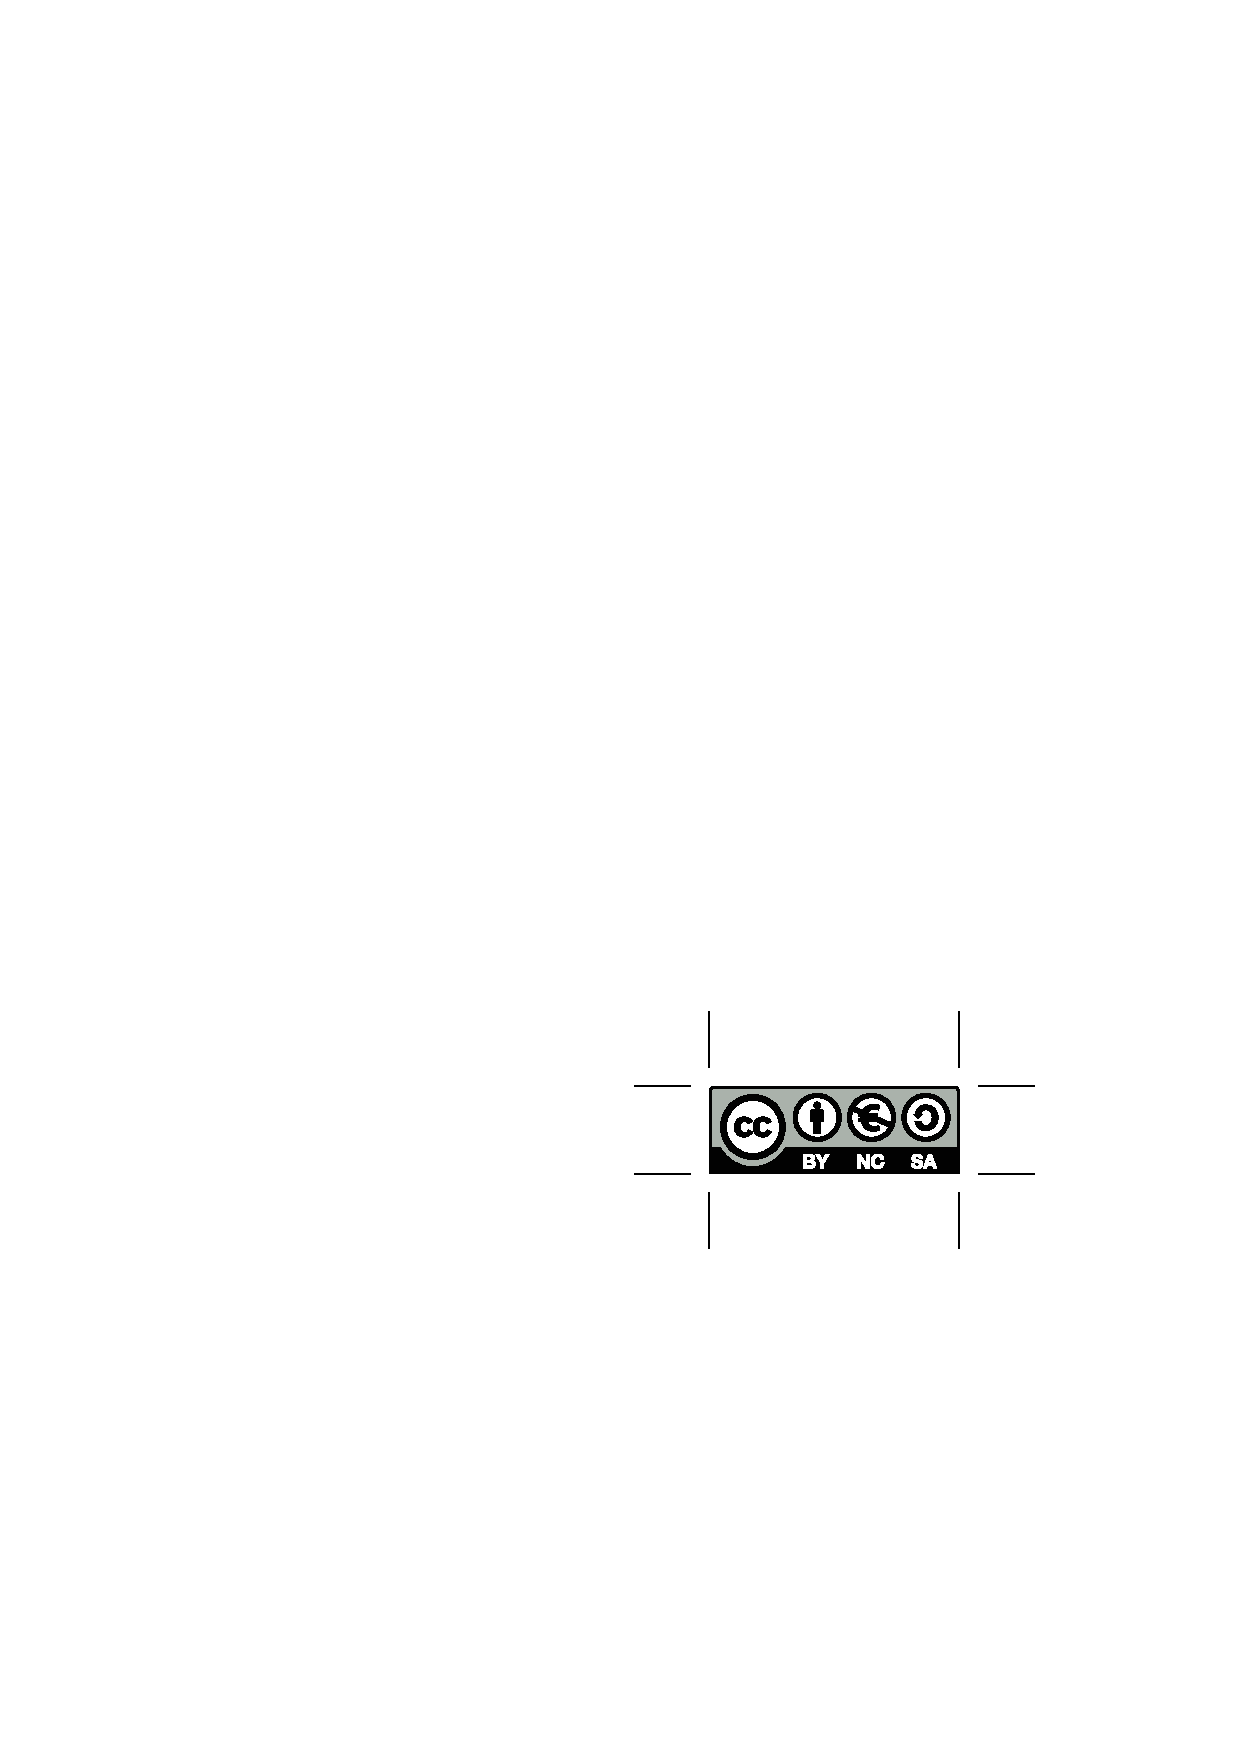
\includegraphics{by-nc-sa}  % Licencia.
\end{center}
\newpage
\tableofcontents    % Índice
\newpage




\section{Números complejos}
\begin{ejer}
	Probar que el conjunto de matrices
	$$ M = \left\{ 
	\left( \begin{array}{cc}
	 a & b \\
	-b & a \end{array} \right)
	: \ a, b\in \mathbb{R}\right\} $$
	con las operaciones de suma y producto de matrices, es un cuerpo isomorfo a $\mathbb{C}$.
\end{ejer}


\begin{ejer}
	Calcular la parte real, la parte imaginaria y el módulo de los números complejos
	$$ \frac{i-\sqrt{3}}{1+i}\hspace{1cm}\text{y}\hspace{1cm} \frac{1}{i\sqrt{3}-1} $$
\end{ejer}



\begin{ejer}
	Sea $U=\{ z\in\mathbb{C} : |z|<1 \}$.
	Fijado $a \in U$, se considera la función $f: U\rightarrow\mathbb{C}$ dada por
	$$ f(z) = \frac{z-a}{1-\overline{a}z}\hspace{1cm} \forall z\in U $$
	Probar que $f$ es una biyección de U sobre sí mismo y calcular su inversa.
\end{ejer}

\begin{sol}

$$|f(z)| < 1 \hspace{1cm} \forall z\in\mathbb{C} \text{ tal que } |z| <1$$
$$f^{-1}(z)= \frac{z+a}{1+\overline{a}z}$$
Si $|z|=1$, entonces $$|f(z)| = 			
	\left|\frac{z-a}{1-\overline{a}z}\right|$$
multiplicando en esta expresión por $\overline{z}$
$$ \frac{z-a}{1-\overline{a}z} \overline{z}  =  \frac{1-a\overline{z}}{1-\overline{a}z}$$
Tenemos entonces que $f$ es holomorfa en el disco $D(0,1)$, lleva la frontera en la frontera.
\end{sol}


\begin{ejer}
	Dados $z_1, z_2, \ldots , z_n \in C^{\ast}$, encontrar una condición necesaria y suficiente para que se verifique la siguiente igualdad:
	$$ \left|\sum_{k=1}^n z_k\right| = \sum_{k=1}^n |z_k|$$
\end{ejer}


\begin{sol}



Por inducción, todos los números complejos deben tener el mismo argumento, son vectores linealmente dependientes sin que se invierta el signo de ninguno de ellos.
$$\exists\lambda_1,...,\lambda_n>0 : \lambda_1 z_1 = \lambda_2 z_2 = ... = \lambda_n z_n$$
para probar que es necesaria no hace falta hacer inducción
$$ \left|\sum_{k=1}^n z_n\right| 
=
\left|\sum_{k=1}^n \frac{\lambda_1}{\lambda_k} z_1\right| 
=
|z_1|\sum_{k=1}^n \frac{\lambda_1}{\lambda_k} 
=
|z_1|\sum_{k=1}^n \frac{|z_k|}{|z_1|} 
=
\sum_{k=1}^n |z_k|$$
Sabemos que en el caso $n=2$
$$|z_1+z_2| = |z_1| + |z_2| \Longleftrightarrow z_2 = \lambda z_1\text{ con }\lambda \in \mathbb{R}$$
Sea cierto para $n\in\mathbb{N}$
$|\sum_{k=1}^{n+1} z_k| 
=
|z_{n+1} + \sum_{k=1}^n z_k|
=
|z_{n+1}| + |\sum_{k=1}^n z_k|$

Donde en este último paso hemos usado que
$$|z_{n+1}|+\left|\sum_{k=1}^nz_n\right| 
\geq 
\left|\sum_{k=1}^{n+1} z_k\right|=\sum_{k=1}^{n+1} |z_k| = |z_{n+1}| + \sum_{k=1}^n |z_k|$$
donde la otra desigualdad entre los extremos se sabe de la desigualdad triangular.
Vemos que
$$|z_{n+1}| + \left|\sum_{k=1}^n z_k\right| 
=
|z_{n+1}| + \sum_{k=1}^n |z_k|$$
Por la hipótesis de inducción para $k=2$, tenemos que 
$$\exists \lambda >0 : z_{n+1} = \lambda \sum_{k=1}^n z_k$$
Nos queda por hacer lo análogo con el resto de números complejos $z_k,k=1...n$
Por la hipótesis de inducción para $k=n, \exists \mu_1,...\mu_n : \mu_1 z_1 = \mu_2 z_2=...= \mu_n z_n$,
como $z_{n+1} = \lambda \sum_{k=1}^n z_k 
=
\lambda \sum_{k=1}^n \frac{\mu_1}{\mu_k} z_1$
$$ |z_1+z_2| = |z_1|+|z_2| 
\Longleftrightarrow
|z_1+z_2|^2 = (|z_1|+|z_2|)^2 
=
|z_1|^2 + 2|z_1||z_2|+|z_2|^2$$
 entonces tenemos
$$z_1 \overline{z_2}=\lambda>0 \hspace{0.5cm}\text{ y }\hspace{0.5cm} z_1 = \frac{\lambda}{|z_2|^2 }z_2 
$$

\end{sol}

\begin{ejer}
	Describir geométricamente los subconjuntos del plano dados por
	$$ A=\{ z\in\mathbb{C} : |z+i|=2|z-i| \} \text{ y } B=\{ z\in\mathbb{C} : |z-i| + |z+i| = 4 \} $$
\end{ejer}

\begin{sol}

\

Veamos el conjunto A, notamos $z=(a,b)$,
$$ \sqrt{a^2+(b+1)^2} = 2\sqrt{a^2+(b-1)^2}$$
Entonces $$a^2+b^2+1+2 b = a^2+(b+1)^2 = 4(a^2+(b-1)^2) = 4a^2+4b^2+4-8b$$
Luego
$$3a^2+3b^2-10b+3=0 \implies a^2+b^2-\frac{10}{3}b+1=0$$
Sumamos y restamos $\frac{25}{9}$
$$a^2+\left(b-\frac{5}{3}\right)^2-\frac{25}{9}+1 \implies a^2+(b-\frac{5}{3})^2=\frac{16}{9}$$
Por lo tanto $A$ es la circunferencia con $c=(0,5/3)$ y radio $r=\frac{4}{3}$

\

Veamos el B, elevando dos veces al cuadrado tenemos como resultado una elipse
$$ \frac{a^2}{\sqrt{3}^2} + \frac{b^2}{2^2} = 1 $$
\end{sol}



\begin{ejer}
	Probar que $arg(z) = 2\arctan\left( \frac{Im(z)}{Re(z) + |z|} \right)$ para todo  $z\in\mathbb{C}^{\ast}\backslash\mathbb{R}^{-}$.
\end{ejer}

\begin{sol}

Usamos la fórmula del ángulo doble
$$ \cos(2\alpha) = \cos^2(\alpha)-\sin^2(\alpha) \hspace{1cm} \sin(2\alpha) = 2\sin(\alpha)\cos(\alpha) $$
$\phi = \arctan\left(\frac{Im z}{Re z + |z|}\right) \implies \phi = 2\alpha = \arctan\left(\frac{Im z}{Re z + |z|}\right) $

\textbf{Pista para otra forma de hacerlo}
$$ \phi = 2\arctan ( \frac{Im z}{Re z + |z|} ) 
|z|(\cos(\phi)+i\sin(\phi)) =? z $$
Para ello usamos, si $t=\theta/2$
$$ \cos(\theta) = \frac{1-\tan^2(\theta/2)}{1+\tan^2(\theta/2)}
\sin(\theta) = \frac{2\tan(\theta/2)}{1+\tan^2(\theta/2)} $$
\end{sol}


\begin{ejer}
	Probar que, si $z=x+iy\in\mathbb{C}^{\ast}$, con $x,y\in\mathbb{R}$, se tiene
	
	$$
	arg(z) = \left\{ 
		\begin{array}{lcc}
			\arctan(y/x) &   si  & x>0 \\
			\arctan(y/x) + \pi & si & x<0, y>0 \\
			\arctan(y/x)-\pi & si & x<0,y<0 \\
			\pi/2 & si & x=0,y>0 \\
			-\pi/2 & si & x=0,y<0 
		\end{array}
	\right.
	$$
\end{ejer}


\begin{ejer}
	Probar las \textit{fórmulas de De Moivre}:
	$$ \cos(n\theta) + i\sin(n\theta) = (\cos(\theta)+i\sin(\theta))^n \hspace{1cm}\forall\theta\in\mathbb{R}, \forall n\in\mathbb{N} $$
\end{ejer}


\begin{sol}
Haremos la prueba por inducción, para el caso inicial $n=1$ es trivial, suponemos cierto para un $n\in\mathbb{N}$ genérico.
Probamos que en ese caso es cierto para $n+1$.
$$ 
\cos((n+1)\theta)+i\sin((n+1)\theta) 
=
\cos(n\theta+\theta)+i\sin(n\theta+\theta)
$$
$$ =
\cos(n\theta) \cos(\theta)- \sin(n\theta)\sin(\theta) +i\cos(n\theta)\sin(\theta) + i\sin(n\theta)\cos(\theta) $$
$$ =
\cos(n\theta)(cos(\theta)+i\sin(\theta)) + i\sin(n\theta)(cos(\theta)+i\sin(\theta))
$$
$$=
(\cos(\theta)+i\sin(\theta)) (\cos(n\theta)+i\sin(n\theta))
=
(cos(\theta)+i\sin(\theta))^{n+1}
$$
La última igualdad la tenemos por la hipótesis de inducción.
\end{sol}



\begin{ejer}
	Calcular las partes real e imaginaria del número complejo 
	$\left( \frac{1+i\sqrt{3}}{2} \right)^8$
\end{ejer}


\begin{ejer}
	Probar que, para todo $x\in\mathbb{R}$, se tiene
	\begin{enumerate}[label=(\alph*)]
		\item $\sin\left( \frac{x}{2} \right) \sum_{k=0}^{n} \cos(kx) = \cos\left( \frac{nx}{2} \right) \sin\left( \frac{(n+1)x}{2} \right)$
		\item $\sin\left( \frac{x}{2} \right) \sum_{k=1}^n \sin(kx) = \sin\left( \frac{nx}{2} \right)\sin\left( \frac{(n+1)x}{2} \right)$
	\end{enumerate}
\end{ejer}
\begin{sol}


\textbf{Pista}
Probar las dos simultáneamente y usar la fórmula de Moivre
$ \sum_{k=0}^n ( cos(x)+sin(x) )^k $
$$\sin(x/2) \sum_{k=0}^{n} \cos(kx) + i\sin(x/2) \sum_{k=0}^{n} \sin(kx)$$
Sacamos factor común 
$$ \sin(x/2)\left( \sum_{k=0}^{n} \cos(kx)+i\sin(kx) \right) $$
Usamos la fórmula de Moivre
$$ \sin(x/2) \sum_{k=0}^{n} (\cos(x)+i\sin(x))^k $$
Usamos que $x\not\in 2\pi\mathbb{Z}$
$$ \sin(x/2) \frac{1-(\cos(x)+i\sin(x)^{n+1}}{1-(\cos(x)+i\sin(x)} = \sin(x/2) \frac{ 1- (\cos((n+1)x)+i\sin((n+1)x)) }{1 - \cos(x) - i\sin(x)} $$
Usamos que $2\sin^2(x/2) = 1-\cos(x)$ y que $\sin(x) = \sin(x/2)\cos(x/2)$,
$$ 
\sin(x/2) \frac{ 1- (\cos((n+1)x)+i\sin((n+1)x)) }{ 2\sin^2(x/2)-2i\sin(x/2)\cos(x/2) }
=
\frac{ 1- (\cos((n+1)x)+i\sin((n+1)x)) }{ 2\sin(x/2)-2i\cos(x/2) }
 $$
$$
\frac{ 2\sin^2 (\frac{n+1}{x}x)-i2\sin(\frac{n+1}{2}x)\cos(\frac{n+1}{2}x) }{ 2\sin(x/2) -2i\cos(x/2) }
$$
Multiplicamos numerador y denominador por el conjugado del denominador
$$
\sin\left(\frac{n+1}{2}x\right)\left(
\sin\left(\frac{n+1}{2}x\right)-i\cos\left(\frac{n+1}{2}x\right) \right)( \sin(x/2)+i\cos(x/2) )
$$
$$ 
=  \sin\left(\frac{n+1}{2}x\right) \left( \cos\left(\frac{n+1}{2}x\right)\cos(x/2) + \sin\left(\frac{n+1}{2}x\right)\sin(x/2)  + i\left( \sin\left(\frac{n+1}{2}x\right)\cos(x/2) - \cos\left(\frac{n+1}{2}x\right)\sin(x/2) \right) \right)
$$
$$ = \sin\left(\frac{n+1}{2}x\right) \left(\cos\left(\frac{nx}{2}\right) + i\sin(\frac{nx}{2})\right)
$$
\end{sol}

\newpage

\section{Topología del plano complejo}
\begin{ejer}
	Estudiar la continuidad de la función argumento principal, $\arg : \mathbb{C}^{\ast} \rightarrow \mathbb{R}$.
\end{ejer}

\begin{sol}


Usamos la fórmula de la relación anterior para probar que es continua en $\mathbb{C}^{\ast} \backslash \mathbb{R}$
$$  
arg z = 2\arctan \left(\frac{Imz}{Rez + |z|}\right) \hspace{1cm} \forall z\in\mathbb{C}^{\ast}\backslash\mathbb{R}
$$
Luego nos aproximamos por sucesiones
$$  
\left\{ z+\frac{i}{n} \right\} \rightarrow z \hspace{1cm}
\lim_{n\rightarrow\infty}\left(arg\left(z+\frac{i}{n}\right)\right) = \lim_{n\rightarrow\infty}\left( \arctan\left(\frac{1}{nz}+\pi\right) \right) = \pi
$$
$$
\left\{ z-\frac{i}{n} \right\} \rightarrow z \hspace{1cm}
\lim_{n\rightarrow\infty}\left(arg\left(z-\frac{i}{n}\right)\right) = \lim_{n\rightarrow\infty}\left( \arctan\left(\frac{-1}{nz}-\pi\right) \right) = -\pi
$$
Como los límites no coinciden no existe dicho límite y la función no es continua.
\end{sol}

\begin{ejer}
	Dado $\theta\in\mathbb{R}$, se considera el conjunto $S_{\theta} = \{ z\in\mathbb{C}^{\ast} : \theta\not\in Arg(z) \}$. 
	Probar que existe una función $\varphi\in\mathcal{C}(S_{\theta})$ que verifica $\varphi(z)\in Arg(z)$ para todo $z\in S_{\theta}$
\end{ejer}

\begin{sol}
Definimos
$$
f(z) = z( \cos(\pi-\theta) + i\sin(\pi-\theta) ) \hspace{2cm} f:\mathbb{C}\rightarrow \mathbb{C} \text{ continua}
$$
$$
\phi(z) = arg(f(z)) - (\pi-\theta) \hspace{2cm} \phi: S_{\theta} \rightarrow \mathbb{C} \text{ continua}
$$
$$ 
\phi(z) \in Arg (f(z)) + \theta-\pi \subset Arg (f(z)) + Arg( \cos(\theta-\pi)+i\sin(\theta-\pi) ) 
$$
$$= Arg ( f(z)-\cos(\theta-\pi)+i(\theta-\pi) ) = Argz
$$
\end{sol}

\begin{ejer}
	Probar que no existe ninguna función $\phi\in\mathcal{C}^{\ast}$ tal que $\varphi(z)\in Arg(z)$ para todo $z\in\mathcal{C}^{\ast}$, y que el mismo resultado es cierto, sustituyendo $\mathbb{C}^{\ast}$ por $\mathbb{T}=\{ z\in\mathbb{C} : |z|=1 \}$
\end{ejer}

\begin{sol}
$\mathbb{T}$ compacto y conexo $\implies \phi(\mathbb{T})$ es un intervalo cerrado y acotado

Sea $\alpha\in\mathbb{T} : \phi(\alpha) \not =\min(\phi(\mathbb{T})), \max(\phi(\mathbb{T}))$ 
$\phi ( \mathbb{T}-\{ \alpha \} )$ conexo $\implies [ \min(\phi(\mathbb{T})), \phi(\alpha)[ \cup ]\phi(\alpha), \max( \phi(\mathbb{T}) ) ] $ que es una contradicción.

Si $\exists h:\mathbb{C}^{\ast} \rightarrow \mathbb{R}$ con $h(z)\in Arg(z)$ $\forall z\in\mathbb{C}^{\ast}$ y $h$ continua, entonces
$h_{| \mathbb{T}} : \mathbb{T} \rightarrow \mathbb{R}$ es continua y $h_{|\mathbb{T}} (z) \in Arg(z) \ \forall z\in\mathbb{T}$
\end{sol}

\begin{ejer}
	Probar que la función $Arg : \mathbb{C}^{\ast} \rightarrow \mathbb{R}\backslash \mathbb{R}/2\pi\mathbb{Z}$ es continua, considerando en $\mathbb{R}/2\pi\mathbb{Z}$ la topología cociente. Más concretamente, se trata de probar que, si $\{z_n\}$ es una sucesión de números complejos no nulos, tal que $\{z_n\} \rightarrow z\in\mathbb{C}^{\ast}$ y $\theta\in Arg(z)$, se puede elegir $\theta_n\in Arg(z_n)$ para todo $n\in\mathbb{N}$, de forma que $\{ \theta_n \} \rightarrow \theta$.
\end{ejer}




\begin{sol}


$$
\{ z_n \} \rightarrow z \implies \forall \epsilon>0\ \exists m\in\mathbb{N} : n\geq m \ |z_n-z|z\epsilon
$$
Sea $\epsilon = \frac{|z|}{2}$, entonces 
$\exists m\in\mathbb{N}$ tal que para $n\geq m$ se tiene $z_n\in D(z, |z|/2)$

A partir de aquí usamos el ejercicio $2$ para concluir.
\end{sol}



\begin{ejer}
	Dado $z\in\mathbb{C}$, probar que la sucesión $\left\{ \left( 1+\frac{z}{n} \right)^n \right\}$ es convergente y calcular su límite.
\end{ejer}


\textbf{Idea}
$$
\left|1+\frac{z}{n}\right|^n \rightarrow e^{Re z}
$$
$$
\lim_{n\rightarrow\infty} \left|1+\frac{z}{n}\right|^n 
= e^{ \lim_{n\rightarrow\infty} n\left(\left|1+\frac{z}{n}\right|-1\right) }
$$
$$
arg\left(\left(1+\frac{z}{n}\right)^n\right) \rightarrow Im z
$$

\begin{sol}


Sea $z_n\in\mathbb{C}$ con$\phi_n\in Arg(z_n)$
$$\{ |z_n| \} \rightarrow |z| \hspace{1cm} \{y_n\} \rightarrow y\in Arg(z)$$
Vamos a usar que is tiene sun sucesión de números complejos y la sucesión de los módulos converge y hay una sucesión de los argumentos de forma que convergen, la sucesión converge al módulo por $cos(x) +isen(x)$

Sabemos que
$$\phi_n \in Arg(z_n)$$
Con lo que tenemos

$z_n = \left(1+\frac{z}{n}\right)^n = \left(1+\frac{a+ib}{n}\right)^n
= \left[\left(1+\frac{a}{n}\right) + \left(\frac{ib}{n}\right)\right] ^n$
$|z_n| = \left[\left| \left(1+\frac{a}{n}\right) + \frac{ib}{n} \right|\right] ^n
= \left[ \left(1+\frac{a}{n}\right)^2 + \left(\frac{b}{n}\right)^n \right]^{1/2}
= lim n \left[ \left(1+\frac{a^2}{n^2} + \left(\frac{a}{n}+\frac{b^2}{n^2}\right) \right)\right]^{n/2}
= e^{  \lim n/2 \left(\frac{a^2}{n^2} + 2a/n + b^2/n^2 \right)  } = e^a = e^{Re z}$ 

Vamos a utilizar la fórmula de Moivre.
%$ z_m = (1+z/n)^n$
$$Arg\left(a+ \frac{a+ib}{n}\right)^n = n Arg\left(a+\frac{a+ib}{n}\right) = n*\arctan \left(\frac{b/n}{1+a/n}\right) = n*\arctan\left(\frac{b}{n+a}\right)$$
Llamamos $y=b/(n+a)$ y usamos $\lim_{y\rightarrow0} \frac{\arctan(y)}{y} = 1$:
$$n*\arctan\left(\frac{b}{n+a}\right) = \frac{\arctan\left(\frac{b}{n+a}\right)}{ \frac{n+a}{n}\frac{b}{n+a}\frac{1}{b} } = b$$
\end{sol}
\newpage

\section{Funciones holomorfas}
\begin{ejer}
	En cada uno de los siguientes casos, estudiar la derivabilidad de la función $f:\mathbb{C} \rightarrow\mathbb{C}$ definida como se indica:
	\begin{enumerate}[label=(\alph*)]
		\item $f(z)  z(Re(z))^2 \hspace{1cm}\forall z\in\mathbb{C}$
		\item $f(x+iy) = x^3 -y+i\left( y^3 +\frac{x^2}{2} \right) \hspace{1cm} \forall x,y\in\mathbb{R}$
		\item $f(x+iy) = \frac{x^3+iy^3}{x^2+y^2} \hspace{1cm} \forall (x,y)\in\mathbb{R}^2\backslash\{(0,0)\}, f(0)=0$
	\end{enumerate}	
\end{ejer}
\begin{sol}

\textbf{a)}
Cauchy Riemman




\textbf{c)}
$$f(x+iy) = \frac{x^3+iy^3}{x^2+y^2}\hspace{0.5cm} \forall (x,y)\in\mathbb{R}^2 \backslash \{ (0,0) \}\hspace{1cm}\text{ con } f(0)=0$$
$$u(x,y) = Re f = \frac{x^3}{x^2+y^2}, \hspace{1cm} v(x,y) = Imf = \frac{y^3}{x^2+y^2}$$
En $\mathbb{C}^{\ast}$ tenemos:
$$ \frac{\partial u}{\partial x} = \frac{3x^2}{x^2+y^2} + \frac{x^4(-1)2}{(x^2+y^2)^2} \hspace{1cm}
\frac{\partial v}{\partial y} = \frac{3y^2}{x^2+y^2} = \frac{y^4(-1)2}{(x^2+y^2)^2}$$
$$ \frac{\partial u}{\partial y} = \frac{x^3 (-1)2y}{(x^2+y^2)^2} \hspace{1cm}
\frac{\partial v}{\partial x} = \frac{y^3(-1)2x}{(x^2+y^2)^2}$$

Usando las ecuaciones de Cauchy-Riemman de las dos primeras ecuaciones deducimos
$$3x^2(x²+y^2) - 2x^4 = 3y^2(x^2+y^2)-2y^4 \implies x^4-y^4 = 0 \implies |x|=|y|$$
de las últimas dos deducimos
$$2yx^3=-2xy^3 \implies xy(x^2+y^2) = 0 \implies xy=0 \text{ ó } x^2+y^2=0$$
Como conclusión, para que la función sea derivable en un punto $x\in\mathbb{C}$ dicho punto debe cumplir que el módulo de su parte real sea igual que el módulo de su parte imaginaria.

\end{sol}



\begin{ejer}
	Probar que existe una función entera $f$ tal que
	$$Re(f(x+iy)) = x^4-6x^2y^2+y^4 \hspace{1cm}\forall x,y\in\mathbb{R}$$
	Si se exige además que $f(0)=0$, entonces $f$ es única.
\end{ejer}
\begin{sol}
Sabemos que dicha función debe satisfacer las ecuaciones de Cauchy-Riemann, así que tenemos
$$ \frac{\partial Re(f)}{\partial x}(x+iy) = 4x^3-12xy^2 = \frac{\partial Im(f)}{\partial y}(x+iy) $$
Integrando con respecto de la variable $y$ el término central nos queda que
$Im(f) = 4x^3*y - 4xy^3+k$ tal que $k\in\mathbb{R}$, ya que también se cumple la condición 
$$ \frac{\partial Re(f)}{\partial y} (x+iy) = -\frac{\partial Im(f)}{\partial x} (x+iy) $$

Si se exige $f(0)=0$ nos queda una única ecuación como resultado de sustituir $k=0$.
\end{sol}

\begin{ejer}
	Encontrar la condición necesaria y suficiente que deben cumplir $a,b,c\in\mathbb{R}$ para que exista una función entera $f$ tal que
	$$ Re(f(x+iy)) = ax^2+bxy+cy^2\hspace{1cm}\forall x,y\in\mathbb{R} $$
\end{ejer}
Usamos Cauchy-Riemann, deben cumplir la condición $a=-c$.


\begin{ejer}
	Sea $\Omega$ un dominio y $f\in\mathcal{H}(\Omega)$. Supongamos que existen $a,b,c\in\mathbb{R}$ con $a^2+b^2>0$, tales que
	$$ aRe(f(z)) + bIm(f(z)) = c\hspace{1cm} \forall z\in\Omega $$
	Probar que $f$ es constante.
\end{ejer}

\begin{sol}

Definimos las funciones $u$ y $v$: 
$Re(f(x+iy)) = u(x,y), \ Im(f(x+iy)) = v(x,y)$

Los casos extremos son $a=0$ o $b=0$, donde o la imagen o la parte real que quedan serían constantes.
$$au(x,y)+bv(x,y)=c \implies -bv(x,y) = c-au(x,y) \implies v(x,y)= c'-a'u(x,y)$$
Derivamos con respecto a $x$ e $y$ a ambos lados de la última ecuación:
$$\frac{\partial v(x,y)}{\partial x} = -a' \frac{\partial u(x,y)}{\partial x} = -a' \frac{\partial v(x,y)}{\partial y} \hspace{1cm} \frac{\partial v(x,y)}{\partial y} = -a' \frac{\partial u(x,y)}{\partial y} = a' \frac{\partial v(x,y)}{\partial x}$$
Con lo que nos queda
$$\frac{\partial u (x,y)}{\partial x} = \frac{\partial v(x,y)}{\partial y} = -a'\frac{\partial v(x,y)}{\partial x}$$
% Quedaba lo siguiente pero creo que está mal
%$$\frac{\partial u (x,y)}{\partial x} = -a'\frac{\partial v(x,y)}{\partial y} = -a'a'\frac{\partial v(x,y)}{\partial x}$$
por tanto
$$\frac{\partial v(x,y)}{\partial x} = 0 = \frac{\partial v(x,y)}{\partial y} \hspace{1cm}\forall (x,y)\in\Omega$$
Como tenemos que la parte imaginaria es constante dentro del dominio $\Omega$ y $f\in\mathcal{H}(\Omega)$, con lo que deducimos que la función $f$ es constante.
\end{sol}



\begin{ejer}
	Sea $\Omega$ un dominio y $f\in\mathcal{H}(\Omega)$. Probar que si $\overline{f}\in\mathcal{H}(\Omega)$, entonces $f$ es constante.
\end{ejer}


\begin{sol}
	
Un dominio es un abierto conexo no vacío.

La función $g := f+\overline{f} = 2Re(f)$ es holomorfa por ser suma de holomorfas, y su parte imaginaria es constante, por tanto $g$ es constante.

Por tanto $Re(f)$ es constante, como $f\in\mathcal{H}(\Omega)$ y $ \Omega$ es un dominio deducimos que $f$ es constante.
\end{sol}





\begin{ejer}
	Sea $\Omega$ un dominio y $f\in\mathcal{H}(\Omega)$. Sea $\Omega^{\ast} = \{ \overline{z} : z\in\Omega \}$ y $f^{\ast}:\Omega^{\ast} \rightarrow \mathbb{C}$ la función definida por
	$$ f^{\ast}(z) = \overline{ f(\overline{z} ) } \hspace{1cm} \forall z\in\Omega^{\ast}$$
	Probar que $f^{\ast}\in\mathcal{H}(\Omega^{\ast})$.
\end{ejer}

\begin{sol}
	
\begin{comment}
% No sé para qué servía esto
Tenemos que 
$P(z) = a_n z^n + a_{n-1}z^{n-1}+...+a_1z + a_0$, 
$P(\overline{z}) = a_n \overline{z}^n + a_{n-1}\overline{z}^{n-1}+...+a_1\overline{z} + a_0 $

$\overline{ P(\overline{z}) } = \overline{a_n}z^n + \overline{a_{n-1}}z^{n-1}+...+\overline{a_1}z + \overline{a_0}$

$\overline{z}^n = \overline{z} ... \overline{z} = \overline{(z^n)}$

resolvemos
\end{comment}
$$a\in\Omega^{\ast} \Longleftrightarrow \overline{a}\in\Omega$$
$$\lim_{z\rightarrow a} \frac{f^{\ast}(z)-f^{\ast}(a)}{z-a} = \lim_{z\rightarrow a} \frac{\overline{f(\overline{z})} - \overline{f(\overline{a})}}{z-a} =
\lim_{z\rightarrow a} \frac{\overline{\overline{f(\overline{z})} - \overline{f(\overline{a})}}}{z-a} =
\lim_{z\rightarrow a} \overline{\left( \frac{f(\overline{z})-f(\overline{a})}{z-a} \right)} =
 \overline{f'(\overline{a})}$$
\end{sol}




\begin{ejer}
	Probar que la restricción de la función exponencial a un subconjunto abierto no vacío del plano, nunca es una función racional. %(*)
\end{ejer}

\begin{sol}

Suponemos que existe dicha función racional:
$$R(z) = \frac{\sum_{i=0}^k \lambda_i z^i}{\sum_{i=0}^m \mu_i z^i} = \frac{A(z)}{B(z)}$$

Usamos que la derivada de la exponencial es ella misma:
$$R(z) = R'(z) = \frac{A'(z)B(z)-A(z)B'(z)}{B(z)^2} = \frac{A(z)}{B(z)}$$
Entonces
$$A(z) = A'(z) - \frac{A(z)B'(z)}{B(z)} \implies
B(z)A(z) = A'(z)B(z) - B'(z)A(z) \hspace{1cm}\forall z\in D(a,r), a\in\mathbb{C}, r>0$$
Tienes dos polinomios que son iguales en un entorno no vacío de un punto.
%$gr(A(z)) \leq gr(A'(z))$
$$gr(B(z)) + gr(A(z)) \leq \max \{ gr(A'(z)) + gr(B(z)), gr(A(z))+gr(B'(z)) \}$$
Por tanto llegamos a una contradicción, al derivar un polinomio su grado disminuiría, con lo que no puede cumplirse la última desigualdad.
Como nuestra hipótesis no es cierta tenemos que dicha función nunca es una función racional.

\end{sol}
\newpage

\section{Funciones analíticas}
\begin{ejer}
	Calcular el radio de convergencia de las siguientes series de potencias:
	\begin{enumerate}[label=(\alph*)]
		\item $\sum_{n\geq1} \frac{n!}{n^n}z^n$
		\item $\sum_{n\geq 0} z^{2n}$
		\item $\sum_{n\geq 0} 2^nz^{n!}$
		\item $\sum_{n\geq 0} (3+(-1)^n)^nz^n$
		\item $\sum_{n\geq 0} (n+a^n)z^n \ (a\in\mathbb{R}^+)$
		\item $\sum_{n\geq 0} a^{n^2}z^n \ (a\in\mathbb{C})$
	\end{enumerate}
\end{ejer}

\begin{comment}


\textbf{b)} %(*)

$\sum_{n\geq 0} z^{2n} = \sum_{n\geq 0} \alpha_nz^n$
con $\alpha_nz{2n+1} =0, \alpha_{2n} = 1$

Vemos el límite superior de la sucesión
$\limsup |\alpha_n| = 1 \implies R=\frac{1}{1} = 1$
\end{comment}

\begin{sol}


\textbf{c)}
$$\sum_{n\geq 0} 2^nz^{n!}$$
Si $|z|\geq 1$ entonces la serie diverge, en el caso $|z|<1$:
$$\sqrt[n]{|2^nz^{n!}|} = \sqrt[n]{2^n|z|^{n!}} = 2|z|^{(n-1)!}$$
Dicha sucesión tiende a $0$ cuando $n\rightarrow\infty$, por tanto %(*)
$$\sum_{n\geq 0} |2^nz^{n!}| < \infty \implies \sum_{n\geq 0} 2^nz^{n!} < \infty$$ 
Entonces el radio de convergencia de la serie es $R=1$.



\textbf{e)}
$$\sum_{n\geq 0} (n+a^n)z^n \hspace{1cm} a\in\mathbb{R}^+$$
Podríamos separar en dos series, calcular sus radios de convergencia y cogemos el menor:
$$\sum_{n\geq 0} nz^n \hspace{1.5cm}\sum_{n\geq 0} a^nz^n\hspace{1cm} a\in\mathbb{R}^+$$
\begin{comment}
Observamos que $a^n \leq n+a^n \leq (n+1)a^n$,
en los extremos el radio de convergencia es $1/a$, por tanto el radio de convergencia de $n+a^n$ es $1/a$
$$\sum_{n\geq 0} a^n |z|^n \leq \sum_{n\geq 0} (n+a^n)|z|^n \leq \sum_{n\geq 0} (n+1)a^n|z|^n$$
Por tanto el radio de convergencia es $1/a$.
\end{comment}

También podemos usar otros criterios:
$$\lim_{n\rightarrow\infty} \sqrt[n]{n+a^n} = \lim_{n\rightarrow\infty} \frac{(n+1)+a^{n+1}}{n+a^n} $$
por tanto el radio de convergencia buscado es:
$$ R = \left\{ \begin{array}{lcc}
1/a &   si  & a>1 \\
1 &  si & a\leq 1
\end{array}
\right. $$


\begin{comment}
\textbf{f)}
$\sum_{n\geq 0} a^{n^2}z^n,a\in\mathbb{C}$
raíz n-esima 
\end{comment}

\end{sol}

\begin{ejer}
	Conocido el radio de convergencia $R$ de la serie $\sum_{n\geq 0} \alpha_nz^n$, calcular el de las siguientes:
	\begin{enumerate}[label=(\alph*)]
		\item $\sum_{n\geq 0} n^k\alpha_nz^n \ (k\in\mathbb{N} \text{ fijo})$
		\item $\sum_{n\geq0} \frac{\alpha_n}{n!}z^n$	
	\end{enumerate}
\end{ejer}
\begin{sol}

\textbf{a)}

El radio de convergencia no se reduce, podemos comprobarlo utilizando el criterio de la raíz.

\textbf{b)}

Vemos el cociente entre los términos $n+1$ y $n$:
$$ \frac{\alpha_{n+1}/(n+1)!}{\alpha_n/n} = \frac{\alpha_{n+1}}{\alpha_n (n+1)}$$
Tomando límites:
$$ \lim_{n\rightarrow\infty} \frac{\alpha_{n+1}}{\alpha_n (n+1)} = \lim_{n\rightarrow\infty}\frac{\alpha_{n+1}}{\alpha_n}\lim_{n\rightarrow\infty}\frac{1}{n+1} = \frac{1}{R} \lim_{n\rightarrow\infty}\frac{1}{n+1} = 0$$
Por tanto el radio de convergencia de la serie es infinito.
\end{sol}

\begin{ejer}
	Caracterizar las series de potencias que convergen uniformemente en todo el plano.
\end{ejer}
\begin{sol}

Convergen en todo el plano las que a partir de cierto término son 0, o sea, las que son una suma finita

Sea $\sum_{n\geq 0} \alpha_n (z-a)^n$ que converge uniformemente
$$S_n=\sum_{k=0}^{n-1} \alpha_k (z-a)^k \text{ \ converge uniformemente } \Longleftrightarrow S_n \text{ es uniformemente de Cauchy }$$
Lo cual, por definición, es:
$$\forall\epsilon>0,\exists m\in\mathbb{N}: p\geq q\geq n \implies |S_p(z)-S_q(z)| < \epsilon \hspace{1cm}\forall z\in\mathbb{C}$$
Sea un polinomio $p\in\mathbb{P}[\mathbb{C}]$, tenemos que $$\lim_{|z|\rightarrow\infty} p(z) = \infty \Longleftrightarrow gr(p)>0 \text{ (grado del polinomio)}$$

Vemos que $|S_p(z)-S_q(z)|$ es un polinomio que está acotado, tiene que ser constante para no diverger en infinito, en particular es la constante $0$, ya que $S_p(a)=S_q(a)$, por tanto $$\sum_{q=m}^{p-10} \alpha_n (z-\alpha)^n = 0 \implies  \alpha_n=0 \hspace{1cm}\forall n\geq m$$ %(*)

\end{sol}

\begin{ejer}
	Estudiar la convergencia puntual, absoluta y uniforme, de la serie $\sum_{n\geq 0} f_n$ donde
	$$ f_n(z) = \left( \frac{z-1}{z+1} \right)^n\hspace{1cm} \forall z\in\mathbb{C}\backslash\{-1\} $$
\end{ejer}

\begin{comment}
Idea:

llamar w a (w-1)/(z-1), y mirar cuando la función tiene imagen que cae en el disco de centro 0 y radio 1, afinar para saber cuando un subconjunto de C po esta función cae dentro de un subconjunto compacto donde el sumatorio converja
\end{comment}
\newpage

\section{Funciones elementales}
\begin{ejer} %(*)
	Sea $f:\mathbb{C}\rightarrow\mathbb{C}$ una función verificando que
	$$ f(z+w) = f(z)f(w) \hspace{1cm} \forall z,w\in\mathbb{C} $$
	Probar que, si $f$ es derivable en algún punto del plano, entonces $f$ es entera. Encontrar todas las funciones enteras que verifiquen la condición anterior. Dar un ejemplo de una función que verifique dicha condición y no sea entera.
\end{ejer}

\begin{sol}
Vemos los posibles valores de $f(0)$
$$f(0) = f(0+0) = f(0)^2 \implies f(0)= 0 \text{ ó }f(0) = 1$$
Si $f(0)=0$ la función es constante, si es $f(0)=1$ y suponiendo que $f$ es derivable en $\alpha\in\mathbb{C}$:

$\exists \lim_{h\rightarrow 0} \frac{f(\alpha+h)-f(\alpha)}{h}$
vemos que cumple la fórmula de adición 
$$f'(\alpha) = \lim_{h\rightarrow 0}\frac{f(\alpha+h)-f(\alpha)}{h} = \lim_{h\rightarrow 0}f(\alpha) \frac{f(h)-f(0)}{h} \Longleftrightarrow f \text{ es derivable en } 0$$ y eso se puede aplicar $\forall z\in\Omega$ de la siguiente forma:
$$ \lim_{h\rightarrow 0}\frac{f(y+h+0)-f(y+0)}{h} = \lim_{h\rightarrow 0} \frac{f(y)f(h+0)-f(y)f(0)}{h} = f(y)\lim_{h\rightarrow 0} \frac{f(h+0)-f(0)}{h} =f(y)f'(0)  $$

Ahora encontramos todas las funciones enteras que cumplan la condición del enunciado.

Sea $z\in\Omega$, $f(z)=0$, $f(z) = e^{wz} : w\in\mathbf{C}$

Sea $f$ tal que $f\in\mathcal{H}(\mathbb{C})$,
$ f'(z) = f(z) \lim_{h\rightarrow 0} \frac{f(h)-f(0)}{h}$
$$(f(z) e^{-wz})' = f'(z) e^{-wz} + (-w) +ze^{-wz} = f(z)we^{-wz} - f(z)we^{-wz} = 0$$
Por lo que las funciones son iguales salvo una constante.
En el punto $0$ las dos funciones valen lo mismo, por lo que la función es la constante $1$, ya que $f(0)=1$


El ejemplo de función entera que verifique dicha condición es $f(z) = e^{Re(z)}$
\end{sol}


\begin{ejer}
	Calcular la imagen por la función exponencial de una banda horizontal o vertical y del dominio cuya frontera es un rectángulo de lados paralelos a los ejes.
\end{ejer}

\begin{sol}

Podemos ver la exponencial como $e^z = e^{Re(z)} (\cos(Imz) + i\sin(Imz))$, sean $a,b\in\mathbb{R}$ con $a<b$.
Definimos las bandas horizontales y verticales:
$$B_H = \{ z\in\mathbb{C} : a\leq Rez \leq b \} \hspace{1cm} B_V = \{ z\in\mathbb{C} : a\leq Imz \leq b \}$$
Si $a\leq Rez \leq b$, $e^a \leq e^{Rez} \leq e^b$
la función se mueve por toda la circunferencia.%? unidad.

Cuando la parte imaginaria se puede mover donde quiera le das infinitas vueltas a la circunferencia unidad. Tenemos que
$exp(B_H)$ es la corona circular de centro $0$ y radios $e^a$ y $e^b$.

Tenemos que $\exp(B_V)$ es el sector del plano encerrado entre los ángulos $a$ y $b$.

En el caso del dominio cuya frontera es un rectángulo de lados paralelos a los ejes su imagen quedaría una corona restringida a los ángulos determinados por la parte imaginaria de dicho rectángulo.


\end{sol}


\begin{ejer}
	Dado $\theta\in]-\pi,\pi[$, estudiar la existencia del límite en $+\infty$ de la función $\varphi : \mathbb{R}^+\rightarrow\mathbb{C}$ definida por $\varphi(r) = exp(re^{i\theta})$ para todo $r\in\mathbb{R}^+$.
\end{ejer}



\begin{ejer}
Probar que si $\{z_n\}$ y $\{w_n\}$ son sucesiones de números complejos, con $z_n \not = 0$ para todo
$n\in \mathbb{N}$ y $\{ z_n \} \rightarrow 1$, entonces
$$ \{w_n(z_n-1)\} \rightarrow \lambda\in\mathbb{C} \implies \{ z_n^{w_n} \}\rightarrow e^{\lambda} $$
\end{ejer}

\begin{sol}

Como la función exponencial es continua
$\{ w_n (z_n-1) \} \rightarrow \lambda \implies \{ e^{w_n(z_n-1)} \} \rightarrow e^{\lambda}$
$$\lim \{ \log(z_n) \} = 0 \implies \lim \{ z_n-\log(z_n) \} = 1 \implies \lim \{ w_n(z_n-\log(z_n))-w_n \} = 0$$
$$\lim \left\{ z_n^{w_n} = e^{\log(z_n)-w_n} \right\}= \lim \left\{ e^{w_n (z_n-1)} \right\} \Longleftrightarrow \lim\left\{ \frac{e^{w_n(z_n-1)}}{e^{w_n (\log(z_n))}} = e^{w_n (z_n-\log(z_n))-w_n} \right\} = 1$$
Vemos que
$$z_n^{w_n} = e^{w_n \frac{\log(z_n)}{z_n-1} (z_n-1)} =  e^{w_n (z_n-1) \frac{\log(z_n)}{z_n-1}}$$
Y sabemos que $ \frac{\log(z_n)}{z_n-1} \rightarrow 1$ ya que
$\lim_{z\rightarrow 1} \frac{\log(z)-\log(1)}{z-1} = \log'(1) = 1/1$

\end{sol}




\begin{ejer}
	Estudiar la convergencia puntual, absoluta y uniforme de la serie de funciones $\sum_{n\geq 0} e^{-nz^2}$
\end{ejer}

\begin{sol}
La serie converge puntualmente si, y sólo si, $\left| \frac{1}{e^{z^2}} \right| <1$, además
$$\left| \frac{1}{e^{z^2}} \right| <1 \Longleftrightarrow 1<|e^{z^2}|  \Longleftrightarrow 0<Rez^2 = (Rez)^2-(Imz)^2 
\Longleftrightarrow |Rez| > |Imz|$$
donde en la última implicación hemos usado
$e^{z^2} = e^{Rez^2} e^{Imz^2}$
$$Rez^2 = (Rez)^2 - (Imz)^2 \hspace{1cm}Rez^2>0 \Longleftrightarrow |Rez| > |Imz|$$
Vemos ahora la convergencia uniforme, definimos
$$A = \{ z\in\mathbb{C} : (Rez)^2>(Imz)^2 \}$$
Si un conjunto $B\subset A$ y satisface que $\inf_{z\in B} [ (Rez)^2-(Imz)^2 ] > 0$, entonces hay convergencia uniforme en $B$.
\end{sol}



\begin{ejer}
	Probar que $a, b, c \in\mathbb{T}$ son vértices de un triángulo equilátero si, y sólo si, $a+b+c = 0$.
\end{ejer}

\begin{sol}
Para que los vértices en $\mathbb{T}$ formen un triángulo equilátero deben tener entre ellos una diferencia en el argumento de $2\pi/3$, de esa forma los vértices quedan:
$$\{ a,b,c \} = \{ e^{(\lambda - 2/3\pi)i}, e^{\lambda i}, e^{(\lambda + 2/3\pi)i} \}$$

$\Longrightarrow$
$$e^{2/3\pi i} (a+b+c) = e^{2/3\pi i} a + e^{2/3\pi i}b + e^{2/3\pi i}c = a+b+c \implies a+b+c=0$$

$\Longleftarrow$
$$a'=\frac{a}{a} = 1, b'=\frac{b}{a}, c'=\frac{c}{a} \hspace{1cm} b'=e^{\theta i} , \ \ c' = e^{\gamma i} = -b-1$$
$$a+b+c = 0 \implies a'+b'+c' = 0 \implies 1+b'+c' = 0 \implies c'=-b'-1 \text{ con }\gamma,\theta\in ]-\pi,\pi[$$
De lo que deducimos que 
$(-\cos(\theta)-1)-i\sin(\theta) = (\cos(\gamma)) + i(\sin(\gamma))$, además
$$-\sin(\theta) = \sin(\gamma) \implies \theta = -\gamma 
\hspace{1cm}-\cos(\theta) -1 =  \cos(\gamma)$$
por tanto
$$\theta = \pm\frac{2\pi}{3} = -\gamma$$
\end{sol}




\begin{ejer}
	Sea $\Omega$ un subconjunto abierto no vacío de $\mathbb{C}^{\ast}$ y $\varphi\in\mathcal{C}(\Omega)$ tal que $\varphi(z)^2 = z$ para todo $z\in\Omega$. Probar que $\varphi\in\mathcal{H}(\Omega)$ y calcular su derivada.
\end{ejer}

\begin{sol}
$a\in\Omega$ y vemos que es derivable por la definición
$$\lim_{z\rightarrow a} \frac{\phi(z)-\phi(a)}{z-a} \frac{\phi(z)+\phi(a)}{\phi(z)+\phi(a)} = \lim_{z\rightarrow a} \frac{z-a}{z-a} \frac{1}{\phi(z)+\phi(a)} = \frac{1}{2\phi(a)} = \phi '(a)$$
donde hemos usado que $\phi(a)\not = 0$.

\end{sol}



\begin{ejer}
	Probar que, para todo $z \in D(0, 1)$ se tiene:
	\begin{enumerate}[label=(\alph*)]
		\item $\sum_{n=1}{\infty} \frac{(-1)^{n+1}}{n} z^n = \log(1+z)$
		\item $\sum_{n=1}^{\infty} \frac{z^{2n+1}}{n(2n+1)} = 2z-(1+z)\log(1+z)+(1-z)\log(1-z)$
	\end{enumerate}
\end{ejer}

\begin{sol}

\textbf{a)}
$g = \log (1+z) \in\mathcal{H}(D(0,1))$ y $(\log (1+z))' = \frac{1}{1+z}$ $\forall z\in D(0,1)$

$\frac{1}{1+z} = \frac{1}{1-(-z)} = \sum_{n=0}^{\infty} (-1)^n z^n$
por otra parte la serie de potencias 

$\sum_{n\geq 1} \frac{(-1)^{n+1}}{n} z^n$ tiene radio de convergencia $1$
y su suma $\sum_{n=1}^{\infty} \frac{(-1)^{n+1}}{n} z^n = f(z)$ es holomorfa en $D(0,1)$ y su derivada se calcula término a término
$$f'(z) = \sum_{n=1}^{\infty} \frac{(-1)^{n+1}}{n} n z^{n-1} = \sum_{n=0}^{\infty} (-1)^{n}z^{n}$$
Entonces $f'(z) = g'(z)$ $\forall z\in D(0,1)$, por tanto $f$ y $g$ difieren en una constante.

Como $g(0) = \log(1) = 0 = f(0)$
con lo que tenemos que $f$ y $g$ son iguales en $D(0,1)$

\end{sol}




\begin{ejer}
	Probar que la función $f:\mathbb{C}\backslash\{1,-1\}\rightarrow\mathbb{C}$ definida por
	$$ f(z) = \log\left( \frac{1+z}{1-z} \right) \hspace{1cm} \forall z\in\mathbb{C}\backslash\{1,-1\} $$
	es holomorfa en el dominio $\Omega = \mathbb{C}\backslash\{ x\in\mathbb{R} : |x|\geq 1 \}$ y calcular su derivada. Probar también que
	$$ f(z) = 2\sum_{n=0}^{\infty} \frac{z^{2n+1}}{2n+1} \hspace{1cm} \forall z\in D(0,1) $$
\end{ejer}


\begin{sol}

$f(z) = \log(\frac{1+z}{1-z})$
la función es holomorfa en $\mathbb{C}\backslash \{1\}$
sabemos que $\log \in \mathcal{H}(\mathbb{C}^{\ast}\backslash\mathbb{R}^-)$
y vemos cuando la función logaritmo cae dentro de dicho conjunto

de forma intuitiva
$\frac{1+z}{1-z} \in\mathbb{R}^- \Longleftrightarrow \exists r>0 : z\not=1, \frac{1+z}{1-z} = -r \Longleftrightarrow 1+z = rz-r \Longleftrightarrow z(r-1)=1+r \Longleftrightarrow z = \frac{1+r}{r-1}$

Viendo que
$g(z) = \frac{1+z}{1-z} \in\mathcal{H}(\Omega)$ y $g(\Omega) \subseteq \mathbb{C}^{\ast}\backslash \mathbb{R}^-$
podemos asegurar que $f\in\mathcal{H}(\mathbb{C})$ por composición.
$$f'(z) = \frac{ (1-z+(1+z))/(1-z)^2 }{ (1+z)/(1-z) } = \frac{2}{1-z^2}$$
Siendo $\xi\in\mathcal{H}(\Omega)$, entonces
$\xi '(z) = \frac{1}{1+z} + \frac{1}{1-z} = \frac{2}{1-z^2}$



\textbf{Pista}
hacer $\frac{2}{1-z^2}$ en serie de potencias
\end{sol}





\begin{ejer}
	Sean $\alpha,\beta\in [-\pi,\pi]$ con $\alpha < \beta$ y consideremos el dominio $\Omega = \{ z\in\mathbb{C}^{\ast} : \alpha < arg(z) < \beta \}$. Dado $\rho\in\mathbb{R}^+$ tal que $\rho\alpha,\rho\beta\in[-\pi,\pi]$, probar que definiendo $f(z) = z^{\rho}$ para todo $z\in\Omega$, se obtiene una biyección de $\Omega$ sobre el doninio $\Omega_{\rho} = \{ z\in\mathbb{C}^{\ast} : \rho\alpha < arg(z) < \rho\beta \}$, tal que $f\in\mathcal{H}(\Omega)$ y $f^{-1}\in\mathcal{H}(\Omega_{\rho})$.
\end{ejer}
\textbf{Pista}
$z^{\phi} = e^{ \phi \log z}$ con $\Omega,\Omega_{\phi} \subset \mathbb{C}^{\ast}\backslash \mathbb{R^-}$
$$f^{-1}(z) = \phi^{\frac{1}{\phi\log z}} = z^{1/{phi}}$$


\begin{ejer}
	Estudiar la convergencia de la serie $\sum_{n\geq 0} \frac{\sin(nz)}{2^n}$
\end{ejer}
\textbf{Pista}

$\sin(nz) = \frac{e^{inz}-e^{-inz}}{2i}$, entonces
$\frac{1}{2i} \sum_{n\geq 0} \frac{e^{inz}-e^{-inz}}{2^n}$
Tenemos que ver cuando, para un $z\in\mathbb{C}$ fijo, estudiar la convergencia de las series
$\sum_{n\geq 0} \frac{e^{inz}}{2^n}$ y $\sum_{n\geq 0} \frac{e^{-inz}}{2^n}$

$e^{inz} = e^{in(Rez+iImz)} = e^{-nImz+inRez} = e^{-nImz}e^{inRez}$ con $|e^{inRez}|=1$

$|\frac{e^{inz}}{2^n}| = \frac{e^{-nImz}}{2^n} = (\frac{e^{-Imz}}{2})^n$
entonces

$\sum_{n\geq 0} |\frac{e^{inz}}{2^n}|$ converge $\Longleftrightarrow e^{-Imz} < 2 \Longleftrightarrow -Imz < \ln 2 \Longleftrightarrow -\ln 2 < Imz$

y tenemos convergencia uniforme en $B\subset A= \{ z\in\mathbb{C} : |Imz|<\ln 2 \}$ tal que $\sup_{z\in B} |Imz| < \ln 2$


\begin{ejer}
	Sea $\Omega = \mathbb{C}\backslash\{ x\in\mathbb{R} : |x|\geq 1 \}$. Probar que existe $f\in\mathcal{H}(\Omega)$ tal que $\cos(f(z)) = z$ para todo $z\in\Omega$ y $f(x)==\arccos(x)$ para todo $x\in]-1,1[$. Calcular la derivada de $f$.
\end{ejer}


\begin{ejer}
	Para $z\in D(0,1)$ con $Re(z) \not =0$, probar que
	$$ \arctan\left(\frac{1}{z}\right) + \sum_{n=0}^{\infty} \frac{(-1)^n}{2n+1}z^{2n+1} = \left\{ \begin{array}{lcc}
	\pi/2  &   si  & Re(z)>0 \\
	-\pi/2 &  si & Re(z)<0 \end{array}
	\right. $$
\end{ejer}
\newpage

\section{Integral curvilínea}
\begin{ejer}
	Sean $\alpha\in\mathbb{C}$ y $r\in\mathbb{R}^+$. Probar que $\int_{[\alpha,\alpha+r]}f(z)cdz = \int_{0}^{r} f(\alpha +s)ds$ para cualquier función $f\in C([\alpha,\alpha+r]^{\ast})$. ¿Cuál es la igualdad análoga para un segmento vertical?
\end{ejer}

\begin{sol}

Definimos $\gamma :[0,r] \rightarrow \mathbb{C}, \ \gamma (s) = \alpha + s, s\in[0,r]$
$$\int_{[\alpha,\alpha + r]} f(z)dz = \int_{0}^{r} f(\alpha +s)\gamma ' (s)ds \hspace{1cm}\text{ donde }\gamma ' (s) = 1 \forall s\in [0,r]$$

Para la igualdad respecto a un segmento vertical definimos $\xi : [0,r] \rightarrow \mathbb{C}$, $\xi(s) = \alpha +is \forall s\in[0,r]$
$$\int_{[\alpha,\alpha + ir]} f(z)dz = \int_0^r f(\alpha + is) \gamma ' (s)ds = i\int_0^r f(\alpha +is)ds$$

\end{sol}



\begin{ejer}
	Para $r\in]1,+\infty[$ se define $I(r) = \int_{\gamma_r} \frac{zdz}{z^3+1}$ y $J(r) = \int_{\sigma_r} \frac{z^2e^z}{z+1}dz$ donde $\gamma_r=C(0,r)$ y $\sigma_r = [-r,-r+i]$. Probar que $\lim_{r\rightarrow+\infty} I(r) = \lim_{r\rightarrow+\infty} J(r) = 0$.
\end{ejer}

\begin{sol}
Para la primera integral buscamos una función $M(r)$ de forma que:
$$\left| \int_{\gamma_r} \frac{z}{z^3+1}dz \right| \leq \int_{\gamma_r} \frac{|z|}{|z^3+1|} dz \leq l(\gamma_r)M(r)$$
donde $M(r)>0$ satisface que $\frac{|z|}{|z^3+1|} \leq M(r) \ \ \forall z\in\gamma_r^{\ast}$. Dado $z\in C(0,r)^{\ast}$, $|z| = r $
$$\frac{|z|}{|z^3+1|} \leq \frac{r}{|z^3|-1} = \frac{r}{r^3-1} \implies l(\gamma_r)M(r) = \lim_{r\rightarrow\infty} 2\pi r\frac{r}{r^3-1} = 0$$



Para la segunda integral
$$\left| \int_{\gamma_r} \frac{z^2 e^z}{z+1}dz \right| < \int_{\gamma_r} \frac{|z|^2 |e^z|}{z+1}dz$$

Si $z\in\sigma_r^{\ast}$
$$ |z|^2 = |-r+is|^2 \leq (r+1)^2 \hspace{1cm} s\in[0,1] $$
$$ |z+1| \geq r-1 $$

Como $z\in\sigma_r^{\ast}$, $|e^z| = e^{Rez} = e^{-r}$ y podemos acotar el valor absoluto de la integral por $0$.

\end{sol}


\begin{ejer}
	Probar que $\int_{C(0,r)} \frac{\log(1+z)}{z}dz = 0$ y deducir que $\int_0^{\pi}\log(1+r^2+2r\cos(t))dt = 0$, para todo $r\in]0,1[.$
\end{ejer}

\begin{sol}
Sabemos que $C(0,r)^{\ast} \subset D(0,1)$, definimos $f(z) = \log(1+z)$, $f\in\mathcal{H}(D(0,1))$

Usando la fórmula de Cauchy para la circunferencia (Tema 7):
$$\int_{C(0,r)} \frac{\log(1+z)}{z} dz = f(0)2\pi i = 0$$

Sin usar la fórmula de Cauchy para la circunferencia vemos:
$$\log (1+z) = \sum_{n=1}^{\infty} (-1)^{n+1} \frac{z^n}{n}$$
La serie $\sum_{n\geq 1} (-1)^{n+1} \frac{z^n}{n}$ converge uniformemente sobre compactos de $D(0,1)$ y la sucesión $\{ \frac{1}{z} \}$ está acotada en el compacto $C(0,1)^{\ast}$. 
Por lo tanto 
$\frac{1}{z} \sum_{n\geq 1} (-1)^{n+1} \frac{z^n}{n}$ converge uniformemente en $C(0,r)^{\ast}$ a $\frac{\log (1+z)}{z}$
$$0 = \int_{C(0,r)} \frac{\log(1+z)}{z} dz = \int_{-\pi}^{\pi}  \frac{\log(1+re^{it})}{re^{it}} dt
= i\int_{-pi}^{\pi} \log(1+re^{it}) dt$$
$$i\int_{-\pi}^{\pi} \ln|1+re^{it}|dt -\int_{-\pi}^{\pi} arg(1+re^{it})dt$$
Por tanto
$$ \int_{-\pi}^{\pi} \ln |1+re^{it}|dt = 0$$

Sabemos que 
$$\log(1+re^{it}) = \ln(|1+re^{it}|) + i*arg(1+re^{it})$$
y además
$$\gamma(t) = re^{it}, \gamma:[-\pi,\pi] \rightarrow \mathbb{C}, \ \gamma '(t) = ire^{it}$$


también sabemos que
$$|1+re^{it}| = ((1+r\cos(t))^2 + r^2\sin^2(t))^{1/2} = (1+2r\cos(t) + r^2\cos^2(t) + r^2\sin^2(t))^{1/2} = (1+2r\cos(t)+r^2)^{1/2}$$

por tanto
$$0 = \int_{-\pi}^{\pi} \ln(|1+re^{it}|) dt = 1/2 \int_{-\pi}^{\pi} \ln(1++2r\cos(t) +r^2)dt$$

Como sabemos que el coseno es par
$ 1/2 \int_{-\pi}^{\pi} \ln(1++2r\cos(t) +r^2)dt = \int_{0}^{\pi} \ln (1+2r\cos(t)+r^2) dt$
\end{sol}

\begin{ejer}
	Sea $f\in\mathcal{H}(D(0,1))$ verificando que $|f(z)-1|<1$ para todo $z\in D(0,1)$. Admitiendo que $f'$ es continua, probar que $\int_{C(0,r)} \frac{f'(z)}{f(z)}dz = 0$ para todo $r\in]0,1[$.
\end{ejer}

\begin{sol}
% Sabemos que $f\in D(0,1)$, teniendo que $|f(z)-1|<1, \forall z\in D(0,1)$

Sabemos que $f$ no se anula en $D(0,1)$ (de lo contrario en la integral se dividiría por $0$) y del hecho de que $|f(z)-1|<1$ deducimos que
$f(D(0,1)) \subset D(1,1)$. 
Por tanto $\log(f) \in \mathcal{H}(D(0,1))$

Como $\log(f(z))' = \frac{f'(z)}{f(z)} \implies \frac{f'}{f}$ admite primitiva holomorfa en $D(0,1)$
y $C(0,r) \subset D(0,1)$ es un camino cerrado, por tanto
$$\int_{C(0,r)} \frac{f'(z)}{f(z)}dz = 0$$

\end{sol}

\begin{ejer}
	Sean $\Omega = \mathbb{C}\backslash \{i,-i\}$ y $f\in\mathcal{H}(\Omega)$ dada por $f(z)=1/(1+z^2)$ para todo $z\in\Omega$. Probar que $f$ no admite una primitiva en $\Omega$.
\end{ejer}

\begin{sol}
Sabemos que
$$\frac{1}{1+z^2} = \frac{1}{(z-i)(z+i)} = \frac{A}{z-i} + \frac{B}{z+i} = \frac{1}{2i} \left[ \frac{1}{z-i} - \frac{1}{z+i} \right]$$
Por tanto
$$\int_{C(i,1)} \frac{1}{1+z^2} dz = \frac{1}{2i} \left[ \int_{C(i,1)}\frac{1}{z-i}dz - \int_{C(i,1)} \frac{1}{z+i}dz \right] \not = 0$$

La primera es $2\pi i$ y la segunda integral es $0$ por el teorema de Cauchy para dominios estrellados (Tema 7), teniendo que $C(i,1) \subset D(i,3/2)$.
\end{sol}


\begin{ejer}
	Probar que $\int_{\sigma} \frac{dz}{1+z^2} = 0$, donde $\sigma(t) = \cos(t)+(i/2)\sin(t)$ para todo $t\in[0,2\pi]$.
\end{ejer}
\textbf{Idea}

$\Omega = \mathbb{C}\backslash \{ iy : |y|>1 \}$
$\arctan \in \mathcal{H}(\Omega)$ y $\arctan$ es una primitiva de $\frac{1}{1+z^2}$

$\sigma ^{\ast} \subset \Omega$ y $\sigma$ es un camino cerrado.

Con esa información sabremos que 
$\int_{\sigma} \frac{1}{1+z^2} dz = 0$


\newpage

\section{Teorema local de Cauchy}

\begin{ejer}
	Sean $a\in\mathbb{C}$ y $r\in\mathbb{R}^+$. Probar que para $z\in\mathbb{C}$ con $|z-a|>r$ se tiene
	$$ \int_{C(a,r)} \frac{dw}{w-z} = 0 $$
\end{ejer}
\begin{sol}
Fijo $z\in\mathbb{C}$ con $|z-a|>r, \exists r'>0 : |z-a|>r'>r$.
Consideramos $\Omega = D(a,r'), f(w) = \frac{1}{w-z}$ , $f\in\mathcal{H}(D(a,r'))$. Sabemos que $D(a,r')$ es convexo (en particular estrellado), por tanto, usando el teorema de Cauchy para dominios estrellados tenemos % y $TLC$
$$\int_{C(a,r)} \frac{dw}{w-z} = 0$$
\end{sol}


\begin{ejer}
	Probar la siguiente versión, más general, de la fórmula de Cauchy:
	
	Sean $a\in\mathbb{C},R\in\mathbb{R}^+$ y $f:\overline{D}(a,R) \rightarrow \mathbb{C}$ una función continua en $\overline{D}(a,R)$ y holomorfa en $D(a,R)$. Se tiene entonces:
	$$ f(z) = \frac{1}{2\pi i} \int_{C(a,R)} \frac{f(w)}{w-z}dw \hspace{1cm} \forall z\in D(a,R) $$
\end{ejer}

\begin{sol}

Fijo $z\in D(a,R)$
Fijo $0<r<R : |z-a|<r<R$, $\overline{D}(a,r) \subset D(a,R)$

Por la fórmula de Cauchy para la circunferencia $f(z) = \frac{1}{2\pi i} \int_{C(a,r)} \frac{f(w)}{w-z} dw$
$$ \left|\frac{1}{2\pi i} \int_{C(0,R)} \frac{f(w)}{w-z} dz - \frac{1}{2\pi i} \int_{C(0,r)} \frac{f(w)}{w-z}dw \right| = \frac{1}{2\pi} \left|\int_{-\pi}^{\pi} \frac{f(a+Re^{it}) iRe^{it} }{ a+Re^{it}-z } dt - \int_{-\pi}^{\pi} \frac{f(a+re^{it}) ire^{it}}{a+re^{it}-z} dt\right|$$
$$\leq \frac{1}{2\pi} \int_{-\pi}^{\pi} \left| \frac{f(a+Re^{it})R}{a+Re^{it}-z} -\frac{f(a+re^{it})r}{a+re^{it}-z} \right| dt$$
Definimos
$$g:[r,R]\times]-\pi, \pi[ \rightarrow \mathbb{C} \hspace{1cm}
g(p,t) = \frac{f(a+pe^{it})p}{a+pe^{it}-z}$$
por lo que el término de la integral queda $|g(R,t)-g(r,t)|$. Vemos que $g$ es uniformemente continua por ser una función continua en un compacto.

Dado $\epsilon >0 \ \exists \delta>0 : si \| (p,t)-(p',t') \| _{\infty}<\delta \implies |g(p,t)-g(p',t')| < \epsilon$,
y lo utilizamos para $(p,t)=(R,t)$ y $(p',t')=(r,t)$. Si $|R-r|<\delta$ entonces $|g(R,t)-g(r,t)| < \epsilon$:
$$\frac{1}{2\pi} \int_{-\pi}^{\pi} \left| \frac{f(a+Re^{it})R}{a+Re^{it}-z} -\frac{f(a+re^{it})r}{a+re^{it}-z} \right| dt \leq \frac{1}{2\pi}\epsilon 2\pi = \epsilon$$
Ahora solamente queda hacer que $r\rightarrow R$.

\end{sol}


\begin{ejer}
	Dados $a\in\mathbb{C}, r\in\mathbb{R}^+$ y $b,c\in\mathbb{C}\backslash C(a,r)^{\ast}$, calcular todos los posibles valores de la integral
	$$ \int_{C(a,r)} \frac{dz}{(z-b)(z-c)} $$
	dependiendo de la posición relativa de $b,c$ respecto a la circunferencia $C(a,r)^{\ast}$.
\end{ejer}

\begin{sol}
	Primero dividimos la integral en dos partes
$$\frac{1}{(z-b)(z-c)} = \frac{1}{b-c} \left[\frac{1}{z-b}-\frac{1}{z-c}\right]$$

Vemos primero el caso $b\not = c$, tendríamos tres subcasos:
\begin{itemize}
	\item b interior, c exterior, la segunda parte es $0$ por el ejercicio $1$
	$$\int_{C(a,r)} \frac{dz}{(z-b)(z-c)} = \frac{1}{b-c} \left[ \int_{C(a,r)} \frac{dz}{z-b} - \int_{C(a,r)} \frac{dz}{z-c} \right] = \frac{2\pi i}{b-c} (1 - 0)$$
	
	\item b y c interiores 
	$$\int_{C(a,r)} \frac{dz}{(z-b)(z-c)} =  \frac{1}{b-c}[2\pi i - 2\pi i] = 0$$
	
	\item b y c exteriores, por el ejercicio 1 ambas partes son $0$
	$$\int_{C(a,r)} \frac{dz}{(z-b)(z-c)} = 0-0 = 0$$
\end{itemize}

Ahora vemos el caso $b=c$, se tiene primitiva holomorfa en $\mathbb{C}^{\ast}, \frac{-1}{z-b}$
$$ \int_{C(a,r)} \frac{dz}{(z-b)^2} = 0 $$

\end{sol}


\begin{ejer}
	Calcular las siguientes integrales:
	\begin{enumerate}[label=(\alph*)]
		\item $\int_{C(0,r)} \frac{z+1}{z(z^2+4)}dz \hspace{1cm} (r\in\mathbb{R}^+, r\not =2)$
		\item $\int_{C(0,1)} \frac{\cos(z)dz}{(a^2+1)z-a(z^2+1)} \hspace{1cm} (a\in\mathbb{C}, |a|\not =1)$
	\end{enumerate}
\end{ejer}

\begin{sol}

\textbf{a)}
Tenemos $\int_{C(0,r)} \frac{z+1}{z(z^2+4)} dz$, donde $r\not = 2$, $z\not = \pm 2i$
$$\frac{z+1}{z(z^2+4)} = \frac{A}{z} + \frac{B}{z-2i} + \frac{C}{z+2i}$$
Nos queda $A = 1/4, B=1/8-i/4, C = -1/8+i/4$, por tanto
$$\int_{C(0,r)} \frac{z+1}{z(z^2+4)} dz = \frac{1}{4} \int_{C(0,r)} \frac{dz}{z} 
+ \left(\frac{1}{8}-\frac{i}{4}\right)\int_{C(0,r)} \frac{dz}{z-2i} 
+
\left(-\frac{1}{8}+\frac{i}{4}\right) \int_{C(0,r)} \frac{dz}{z+2i}$$

Tenemos para las dos últimas integrales y $r\not = 2$ dos casos, si $r<2$ ambas integrales son $0$, si $r>2$ ambas integrales valen lo mismo ($2\pi i *1$) y se anulan entre sí. Por tanto
$$\int_{C(0,r)} \frac{z+1}{z(z^2+4)} dz
=
\frac{1}{4}\int_{C(0,r)} \frac{dz}{z} = \frac{2\pi i}{4} = \frac{\pi}{2}$$

\end{sol}


\begin{ejer}
	Dados $a,b\in\mathbb{C}$ con $a\not =b$, sea $R\in\mathbb{R}^+$ tal que $R>\max \{|a|,|b|\}$. Probar que, si $f$ es una función entera, se tiene:
	$$ \int_{C(0,R)} \frac{f(z)dz}{(z-a)(z-b)} = 2\pi i\frac{f(b)-f(a)}{b-a} $$
	Deducir que toda función entera y acotada es constante.
\end{ejer}
\begin{sol}

Como $R>\max\{ |a|, |b| \}$
$$\int_{C(0,R)} \frac{f(z)}{(z-a)(z-b)}dz = \frac{1}{b-a} \left[ \int_{C(0,R)} \frac{f(z)}{z-b}dz - \int_{C(0,R)} \frac{f(z)}{z-a}dz \right]$$

Por el ejercicio $3$ tenemos
$$\frac{f(z)}{(z-a)(z-b)} = \frac{f(z)}{b-a} \left[ \frac{1}{z-b} - \frac{1}{z-a} \right]$$

Por la fórmula de Cauchy para la circunferencia
$$\frac{1}{b-a} \left[ \int_{C(0,R)} \frac{f(z)}{z-b}dz - \int_{C(0,R)} \frac{f(z)}{z-a}dz \right] = 2\pi i\frac{f(b) - f(a)}{b-a}$$

\textbf{Consecuencia}

Si $\exists M>0 : |f(z)|\leq M\ \ \forall z \in \mathbb{C}$
$$\frac{2\pi |f(b)-f(a)|}{|b-a|} = \frac{|2\pi i(f(b)-f(a))|}{|b-a|} 
\leq \int_{C(0,R)} \frac{|f(z)|}{|z-a||z-b|} dz \leq \frac{M}{(R-|a|)(R-|b|)} 2\pi R$$
que tiende a $0$ cuando $R\rightarrow \infty$ ya que $|z-a|\geq R-|a|$ y $|z-b|\geq R - |b|$
\end{sol}
\newpage

\section{Equivalencia entre analiticidad y holomorfía}
\begin{ejer}
	Sea $\gamma$ un camino y $\varphi : \gamma^{\ast} \rightarrow \mathbb{C}$ una función continua. Se define $f:\mathbb{C}\backslash\gamma^{\ast}\rightarrow\mathbb{C}$ por
	$$ f(z) = \int_{\gamma}\frac{\varphi(w)}{w-z}dw \hspace{1cm} \forall z\in\mathbb{C}\backslash\gamma^{\ast} $$
	Probar que $f$ es una función analítica en $\mathbb{C}\backslash\gamma^{\ast}$ y que
	$$ f^{(k)}(z) = k! \int_{\gamma} \frac{\varphi(w)}{(w-z)^{k+1}}dw \hspace{1cm} \forall z\in\mathbb{C}\backslash\gamma^{\ast}, \ \ \forall k\in\mathbb{N} $$
\end{ejer}

\begin{sol}
Definimos
$$\phi (w,z) = \frac{\varphi(w)}{w-z} \hspace{1cm} \phi : \gamma^{\ast}\times\mathbb{C}\backslash \gamma^{\ast} \rightarrow \mathbb{C}$$
Sabemos que $\phi$ es continua por ser composición de funciones continuas. Vemos 
$$\phi_w(z) = \phi(w,z)\hspace{1cm}\phi_w  \in \mathcal{H}(\mathbb{C} \backslash \gamma^{\ast})$$
Por el teorema de holomorfía de una integral dependiente de un parámetro (Tema $10$) $f\in\mathcal{H}(\mathbb{C}\backslash \gamma^{\ast})$.
Podemos proceder también de otra forma, sea $a\in\mathbb{C}\backslash \gamma^{\ast}$ fijo:
$$\lim_{z\rightarrow a} \frac{f(z)-f(a)}{z-a} = \lim_{z\rightarrow a}  \frac{ \int_{\gamma} \frac{\varphi (w)}{w-z}dw  -  \int_{\gamma} \frac{\varphi (w)}{w-a}dw }{z-a} = \lim_{z\rightarrow a} \int_{\gamma} \frac{\varphi(w)((w-a)-(w-z))}{(z-a)(w-z)(w-a)} dw = \lim_{z\rightarrow a} \int_{\gamma} \frac{\varphi (w) dw}{(w-z)(w-a)}$$

Vamos a ver que podemos intercambiar límite e integral. Dado $r\in\mathbb{R}^+$ suficientemente pequeño, definimos
$$\psi : \phi_{| \gamma{\ast}  \times  \overline{D}(a,r)} \rightarrow \mathbb{C} \hspace{1cm} \psi (w,z) = \frac{\varphi (w)}{(w-z)(w-a)}$$
La función $\psi$ es continua en $\gamma^{\ast} \times \overline{D}(a,r)$, como dicho conjunto es compacto, $\phi$ es uniformemente continua en  $\gamma^{\ast} \times \overline{D}(a,r)$ y podemos intercambiar límite e integral.
De esta forma vemos que $f\in\mathcal{H}(\mathbb{C}\backslash \gamma^{\ast})$, y, por la equivalencia entre analiticidad y holomorfía, vemos que $f$ es analítica en $\mathbb{C}\backslash\gamma^{\ast}$.

La fórmula de $f^{(k)}(z)$ la podemos obtener a partir de la \textit{fórmula de Cauchy para las derivadas} teniendo en cuenta que 
$$ f(z) = 2\pi i\varphi(z) $$


%$\frac{\phi (w)}{(w-z)^{k+1}} - \frac{\phi (w)}{(w-a)^{k+1}} = %\phi (w) = \left[ \frac{(w-a)^{k+1} - %(w-z)^{k+1}}{(w-z)^{k+1}(w-a)^{k+1}} \right]$
\end{sol}





\begin{ejer}
	Para $\alpha\in\mathbb{C}$ se define:
	$$ \binom{\alpha}{0}=1\ \text{ y }\ \binom{\alpha}{n}=\frac{1}{n!} \prod_{j=0}^{n-1}(\alpha-j)=\frac{\alpha(\alpha-1)\dots(\alpha-n+1)}{n!} \ \ \hspace{1cm}\forall n\in\mathbb{N}$$
	Probar que
	$$ (1+z)^{\alpha} = \sum_{k=0}^{\infty}\binom{\alpha}{n}z^n \hspace{1cm}\forall z\in D(0,1) $$
\end{ejer}

\begin{sol}
Vemos que la siguiente función es analítica en el disco $D(0,1)$.
$$(1+z)^{\alpha} = e^{ \alpha \log(1+z) } \in\mathcal{H}(D(0,1))$$


Por el \textit{teorema de desarrollo de Taylor} de la exponencial centrada en cero:
$$
%e^{ \alpha \log(1+z) } =
 \sum_{n\geq 0} \frac{f^{n)}(0)}{n!}z^n$$
\end{sol}

\begin{ejer}
	Obtener el desarrollo en serie de Taylor de la función $f$, centrado en el origen, en cada uno de los siguientes casos:
	\begin{enumerate}[label=(\alph*)]
		\item $f(z) = \log(z^2-3z+2) \hspace{1cm}\forall z\in D(0,1)$
		\item $f(z) = \frac{z^2}{(z+1)^2} \hspace{1cm} \forall z\in \mathbb{C}\backslash\{-1\}$
		\item $f(z) = \arcsin(z) \hspace{1cm} \forall z\in D(0,1)$
		\item $f(z) = \cos^2(z) \hspace{1cm} \forall z\in\mathbb{C}$
	\end{enumerate}
\end{ejer}
\begin{sol}

\textbf{a)}
Derivamos
$$f'(z) = \frac{2z-3}{z^2-3z+2} \hspace{1cm}\frac{1}{z^2-3z+2} = \frac{A}{2-z} + \frac{B}{1-z} = \frac{A/2}{1-z/2} + \frac{B}{1-z}$$
Por tanto el desarrollo en serie de potencias de la original se puede conseguir a partir de desarrollo de las dos partes por separado. Como $z\in D(0,1), |z|<1$ podemos usar la fórmula de la suma de una serie geométrica
$$f'(z) = (2z-3) \sum_{n\geq 0} \left(\frac{A}{2} \left(\frac{z}{2}\right)^n + Bz^n\right) = (2z-3)\sum_{n\geq 0} \left(\frac{A}{2^{n+1}} + B\right)z^n = \sum_{n\geq 0} \left(\frac{A}{2^{n}} + 2B\right)z^{n+1} - \sum_{n\geq 0} 3 \left(\frac{A}{2^{n+1}}+B\right)z^n$$

que nos da como resultado 
$$ f'(z) = -\left(\frac{3A}{2}+B\right) + \sum_{n\geq 1} \left(\frac{A}{2^{n+1}} - B \right)z^n $$ %(*)
\end{sol}

\begin{ejer}
	Dado $\alpha\in\mathbb{C}^{\ast}\backslash\mathbb{N}$, probar que existe una única función $f\in\mathcal{H}(D(0,1))$, verificando que
	$$ zf'(z)-\alpha f(z) = \frac{1}{1+z} \hspace{1cm} \forall z\in D(0,1) $$
\end{ejer}

\begin{ejer}
	Probar que existe una única función $f\in\mathcal{H}(D(0,1))$, verificando que $f(0)=0$ y 
	$$ \exp(-zf'(z)) = 1-z \hspace{1cm} \forall z\in D(0,1) $$
\end{ejer}



\begin{ejer}
	Para $z\in\mathbb{C}$ con $1-z-z^2\not =0$ se define $f(z) = (1-z-z^2)^{-1}$. Sea $\sum_{n\geq 1}\alpha_nz^n$ la serie de Taylor de $f$ centrada en el origen. Probar que $\{\alpha_n \}$ es la sucesión de Fibonacci:
	$$ \alpha_0 = \alpha_{1} = 1 \hspace{1cm}\text{ y }\hspace{1cm} \alpha_{n+2} = \alpha_n + \alpha_{n+1} \hspace{1cm}\forall n\in\mathbb{N}\cup\{0\}  $$
	Calcular en forma explícita dicha sucesión.
\end{ejer}
\begin{sol}
Vemos los ceros del denominador
$$f(z) = \frac{1}{1-z-z^2} = \frac{1}{(z-a_1)(z-a_2)} $$
$$z^2+z-1 = 0 \Longleftrightarrow z = \frac{-1\pm \sqrt{5}}{2} \text{\ \ donde \ \ } a_1=\frac{-1+ \sqrt{5}}{2},a_2=\frac{-1- \sqrt{5}}{2}$$
$$f(z) = \frac{1}{(a_1-z)(a_2-z)} = \frac{1}{a_1-a_2}\left[ \frac{1}{a_1-z}-\frac{1}{a_2-z} \right]$$
Expresamos $\alpha_n$ en términos de $a_1$ y $a_2$
$$a_1+a_2 = -1 \hspace{1cm}a_1*a_2=-1 \hspace{1cm}(z-a_1)(z-a_2) = z^2-(a_1+a_2) + a_1a_2$$

$\alpha_{n+2}$ a partir de aquí se puede expresar en términos de $\alpha_n$ y $\alpha_{n+1}$
\end{sol}


\begin{ejer}
	En cada uno de los siguientes casos, decidir si existe una función $f\in\mathcal{H}(\Omega)$ verificando que $f^{(n)}(0)=a_n$ para todo $n\in\mathbb{N}$:
	\begin{enumerate}[label=(\alph*)]
		\item $\Omega = \mathbb{C}, \ \ a_n=n$
		\item $\Omega=\mathbb{C},\ \ a_n=(n+1)!$
		\item $\Omega=D(0,1), \ \ a_n=2^nn!$
		\item $\Omega=D(0,1/2), \ \ a_n=n^n$
	\end{enumerate}
\end{ejer}

\begin{ejer}
	Dados $r\in\mathbb{R}^+,k\in\mathbb{N}$, y $a,b\in\mathbb{C}$ con $|b|<r<|a|$, calcular la siguiente integral:
	$$ \int_{C(0,r)}\frac{dz}{(z-a)(z-b)^k} $$
\end{ejer}

\begin{ejer}
	Calcular la integral $\int_{\gamma}\frac{e^zdz}{z^2(z-1)}$, para $\gamma=C(1/4,1/2), \gamma=C(1,1/2)$ y $\gamma=C(0,2)$.
\end{ejer}

\begin{ejer}
	Dado $n\in\mathbb{N}$, calcular las siguientes integrales:
	\begin{enumerate}[label=(\alph*)]
		\item $\int_{C(0,1)}\frac{\sin(z)}{z^n}dz$
		\item $\int_{C(0,1)}\frac{e^z-e^{-z}}{z^n}dz$
		\item $\int_{C(0,1/2)}\frac{\log(1+z)}{z^n}dz$
	\end{enumerate}
\end{ejer}

\begin{ejer}
	Probar la siguiente \textit{fórmula de cambio de variable} para la integral curvilínea:
	
	\textit{Si $\Omega$ es un abierto del plano, $\gamma$ un camino en $\Omega$ y $\varphi\in\mathcal{H}(\Omega)$, entonces $\varphi\circ\gamma$ es un camino y, para cualquier función $f$ que sea continua en $(\varphi\circ\gamma)^{\ast}$ se tiene:}
	$$ \int_{\varphi\circ\gamma} f(z)dz = \int_{\gamma}f(\varphi(w))\varphi'(w)dw $$
\end{ejer}

\begin{ejer}
	Usar el resultado del ejercicio anterior para calcular las siguientes integrales:
	\begin{enumerate}[label=(\alph*)]
		\item $\int_{C(0,2)}\frac{dz}{z^2(z-1)^2}$
		\item $\int_{C(0,2)}\frac{dz}{(z-1)^2(z+1)^2(z-3)}$
	\end{enumerate}
\end{ejer}

\begin{sol}

\

\textbf{a)}

Definimos la función y el camino
$f(z) = \frac{1}{z^2(z-1)^2}$
$$ \phi(z) = \frac{1}{z} \hspace{1cm} \gamma{\ast} = \mathcal{C}(0,1/2)^{\ast} \hspace{1cm} \gamma(t) = \frac{1}{2}e^{-it} $$
$$ \phi(\gamma(t)) = 2e^{it}\implies \phi(\gamma^{\ast}) = \mathcal{C}(0,2)^{\ast}$$
Por tanto
$$\int_{\mathcal{C}(0,2)} \frac{dz}{z^2(z-1)^2} = \int_{\mathcal{C}(0,1/2)} \frac{1}{ \frac{1}{w^2} (\frac{1}{w}-1)^2} \frac{1}{w^2} dw = \int_{\mathcal{C}(0,1/2)} \frac{w^2dw}{(1-w)^2}$$
\end{sol}
\newpage

\section{Ceros de las funciones holomorfas}
\begin{ejer}
	Sea $f\in\mathcal{H}(D(0,1))$ tal que
	$$ |f(z)| \leq \frac{1}{1-|z|} \hspace{1cm} \forall z\in D(0,1) $$
	Probar que $|f^{(n)}(0)| \leq e(n+1)!$ para todo $n\in\mathbb{N}$.
\end{ejer}

\begin{ejer}
	Sea $f$ una función entera verificando que existen constantes $\alpha,\beta,\rho\in\mathbb{R}^+$ tales que
	$$ z\in\mathbb{C}, \ \ |z|>\rho \implies |f(z)| \leq \alpha |z|^{\beta} $$
	Probar que $f$ es una función polinómica de grado menor o igual que $\beta$.
\end{ejer}

\begin{ejer}
	Sea $f$ una función entera verificando que
	$$ f(z) = f(z+1)=f(z+i) \hspace{1cm} \forall z\in\mathbb{C} $$
	Probar que $f$ es constante.
\end{ejer}

\begin{ejer}
	Sea $f$ una función entera verificando que $f(f(z))=f(z)$ para todo $z\in\mathbb{C}$. ¿Qué se puede afirmar sobre $f$?
\end{ejer}
\begin{sol}
Existe la posibilidad de que $f$ sea constante.

En otro caso, si $f$ no es constante usando el \textit{teorema de Liouville} sabemos que $f(\mathbb{C})$ es denso en $\mathbb{C}$.
Entonces
$\forall z\in f(\mathbb{C})$, $\exists c\in\mathbb{C} : f(c)=z \implies f(z) = f(f(c)) = f(c) = z$


Por tanto
$$f(\mathbb{C}) \cap \mathbb{C} \implies f(z)=z \hspace{1cm}  \forall z\in \mathbb{C}$$
también se puede razonar de la siguiente forma:
$\forall z\in\mathbb{C}, \exists \{z_n\}_{n\in\mathbb{N}}$ tal que 
$$z_n\in f(\mathbb{C}) \forall n\in\mathbb{N} \text{ y }\{z_n\}\rightarrow z \implies \{f(z_n)\}\rightarrow f(z)=z \implies f(z)=z ,\forall z\in\mathbb{C}$$
\end{sol}

\begin{ejer}
	En cada uno de los siguientes casos, decidir si existe una función $f$, holomorfa en un entorno del origen, y verificando que $f(1/n)=a_n$ para todo $n\in\mathbb{N}$ suficientemente grande:
	\begin{enumerate}[label=(\alph*)]
		\item $a_{2n} = 0, \ \ a_{2n-1}=1 \hspace{1cm} \forall n\in\mathbb{N}$
		\item $a_{2n} = a_{2n-1} = \frac{1}{2n} \hspace{1cm} \forall n\in\mathbb{N}$
		\item $a_n = \frac{n}{n+1} \hspace{1cm} \forall n\in\mathbb{N}$
	\end{enumerate}
\end{ejer}

\begin{ejer}
	Enunciar y demostrar un resultado referente al orden de los ceros de una suma, producto o cociente de funciones holomorfas.
\end{ejer}

\begin{ejer}
	Dado un abierto $\Omega$ del plano, probar que el anillo $\mathcal{H}(\Omega)$ es un dominio de integridad si, y sólo si, $\Omega$ es conexo.
\end{ejer}


\begin{ejer}
	¿Qué se puede afirmar sobre dos funciones enteras cuya composición es constante?
\end{ejer}
\begin{sol}
Siendo $f$ y $g$ las funciones cuya composición es constante tenemos que su derivada se anula
$$f'(g(z)) g'(z) = 0 \hspace{1cm} \forall z\in\Omega$$
entonces puede darse
$f'(g)=0$ o $g'=0$
\end{sol}

\begin{ejer}
	Sea $f$ una función entera verificando que $f(z)\rightarrow\infty (z\rightarrow\infty)$. Probar que $f$ es una función polinómica.
\end{ejer}
\begin{sol}
Definimos
$$h(z) = \frac{1}{f(1/z)} \hspace{1cm} \forall z\in\mathbb{C}^{\ast}$$
Sea $R>0$, entonces $\exists w\in\mathbb{C}$ de forma que si $|w|>R$, entonces $|f(w)|>1$.
Si $z\in D(0,1/R)\backslash\{0\}$, $|z|<1/R \Longleftrightarrow 1/|z|>R$, entonces podemos definir
$$h : D(0,1/R)\backslash\{0\} \rightarrow \mathbb{C} \hspace{1cm} h\in\mathcal{H}(D(0,1/R)\backslash\{0\})$$
Como $\lim_{z\rightarrow 0} h(z) = \lim_{z\rightarrow 0} \frac{1}{f(1/z)} = 0$ deducimos por el Teorema de Extensión de Riemman
$h\in\mathcal{H}(D(0,1/R))$ y $h(0)=0$
$$\exists g\in\mathcal{H}(D(0,1/R))) \text{ con }g(0) \not = 0, \ \exists k\in\mathbb{N} \text{ tal que }h(z) = \frac{1}{f(1/z)} = z^k g(z)$$
$ f(1/z) = \frac{1}{z^k}\frac{1}{g(z)}$
donde el valor absoluto del segundo término está acotado, por tanto
$$f(w) = w^k \frac{1}{g(1/w)}$$
Como $g(0)\not = 0 \exists\delta>0$, $\exists C>0$ tal que $D(0,\delta)\subset D(0,1/R)$:
$$|g(z)| \geq C > 0 \ \ \forall z\in D(0,\delta) \implies \frac{1}{|g(z)|} \leq \frac{1}{C} \ \ \forall z\in D(0,\delta) \implies \frac{1}{|g(1/w)|} \leq \frac{1}{C} \ \ \forall x\in \mathbb{C}\backslash \overline{D}(0,1/\delta)$$
$$|f(w)| = |w|^k \frac{1}{g(1/w)} \leq \frac{1}{C}|w|^k \hspace{1cm} \forall w\in \mathbb{C}\backslash\overline{D}(0,1/\delta)$$
por el ejercicio $2$ de esta relación tenemos que $f$ es un polinomio, en particular de grado menor o igual que $k$.
\end{sol}

\begin{ejer}
	Sea $f$ una función entera verificando que
	$$ z\in\mathbb{C}, \ \ |z|=1 \implies |f(z)|=1 $$
	Probar que existen $\alpha\in\mathbb{C}$ on $|\alpha|=1$ y $n\in\mathbb{N}\cup \{0\}$ tales que $f(z) = \alpha z^n$ para todo $z\in\mathbb{N}$.
\end{ejer}
\begin{sol}

\textbf{Pista}

\begin{lema}
	
Si f verifica que $|z|=1 \implies |f(z)|=1$, entonces $f(0)=0$ o $f$ es constante.

\textit{PISTA DEMOSTRACIÓN LEMA}:
$1=|f(z)|^2 = f(z)\overline{f(z)} \forall z\in\mathbb{T}$ 
$1= f(\overline{z})\overline{f(\overline{z})} = f(1/z)\overline{f(\overline{z})}$
\end{lema}


Si hemos probado eso y f es constante es trivial, en caso contrario
$$f(0)=0 \implies \exists g\in\mathcal{H}(\mathbb{C}), \ \exists k\in\mathbb{N} \text{ tal que }g(0) \not =0 \text{ y }f(z) = z^kg(z)\ \forall z\in\mathbb{C}$$
$$1=|f(z)| = |z|^k|g(z)| \hspace{1cm} z\in\mathbb{T}$$
$g$ está en las mismas condiciones que $f$ y por el lema anterior $g$ es constante.
\end{sol}
\newpage

\section{Teorema de Morera y sus consecuencias}
\begin{ejer}
	Sea $\{f_n\}$ una sucesión de funciones continuas en un abierto $\Omega$ del plano, y sea $f:\Omega\rightarrow\mathbb{C}$ otra función continua. Probar que las siguientes afirmaciones son equivalentes:
	\begin{itemize}
		\item $\{f_n\}$ converge uniformemente a $f$ en cada subconjunto compacto de $\Omega$.
		\item Para toda sucesión $\{z_n\}$ de puntos de $\Omega$ que converja a un punto $z\in\Omega$ se tiene que $\{f_n(z_n)\}\rightarrow f(z)$.
	\end{itemize}
\end{ejer}

\begin{ejer}
	Sea $\{f_n\}$ la sucesión de funciones enteras definida por $f_n(z) = z\exp(-n^2z^2/2)$ para cualesquiera $z\in\mathbb{C}$ y $n\in\mathbb{N}$. Probar que $\{f_n\}$ converge uniformemente en $\mathbb{R}$ pero no converge uniformemente en ningún entorno del origen.
\end{ejer}

\begin{ejer}
	Probar que la serie de funciones $\sum_{n\geq 1} f(z^n)$ converge en $D(0,1)$ y que su suma es una función holomorfa en $D(0,1)$.
\end{ejer}

\begin{ejer}
	Sea $f\in\mathcal{H}(D(0,1))$ tal que $f(0)=0$.
	Probar que la serie $\sum_{n\geq 1}f(z^n)$ converge en $D(0,1)$ y que su suma es una función holomorfa en $D(0,1)$.
\end{ejer}

\begin{ejer}
	Probar que la sucesión de funciones enteras definida por
	$$ f_n(z) = \frac{1}{n}\sin(nz) \hspace{1cm} \forall z\in\mathbb{C}, \ \ \forall n\in\mathbb{N} $$
	converge uniformemente en $\mathbb{R}$ pero no converge uniformemente en ningún subconjunto de $\mathbb{C}$ que tenga interior no vacío.
\end{ejer}
\begin{sol}
Sea $U\subset \mathbb{C}$ con interior no vacío, entonces $\exists z_o\in U, \exists r\in\mathbb{R}^+$ con $|Im(z_o)| \geq r > 0$
$$\frac{1}{n}|\sin(nz_0)| = \frac{1}{n}\left| \frac{e^{inz_0}-e^{-inz_0}}{2i} \right|= \frac{1}{2n} \left| e^{inz_0} - e^{-inz_0} \right|$$
entonces si $Im(z_0)\geq r$
$$\frac{1}{2n} \left| e^{inz_0} - e^{-inz_0} \right|  \geq \frac{1}{2n} \left( e^{nIm(z_0)} -e^{-nIm(z_0)} \right)  $$
que tiende a infinito cuando $n\rightarrow\infty$
\end{sol}

\begin{ejer}
	Probar que la serie $\sum_{n\geq 0} \frac{\sin(nz)}{3^n}$ converge en la banda $\Omega = \{ z\in\mathbb{C} : |Im(z)|<\log(3) \}$ y que su suma es una función $f\in\mathcal{H}(\Omega)$. Calcular $f'(0)$.
\end{ejer}
\begin{sol}
Expresamos el seno en función de la exponencial
$$\frac{\sin(nz)}{3^n} = \frac{1}{2i} \left( \frac{e^{inz}}{3^n} - \frac{e^{-inz}}{3^n} \right)$$
La segunda parte del paréntesis tiene a 0 cuando $n\rightarrow \infty$
$$\left| \frac{e^{inz}}{3^n} \right| = \frac{|e^{inRe(z)-nIm(z)}|}{3^n} =
\frac{e^{nIm(z)}}{3^n} = 
\left( \frac{e^{Im(z)}}{3} \right)^n$$
tenemos que hacer que sea menor que $\delta^n$ con $0<\delta<1$, lo que pasa solamente cuando $-Im(z) < \log(3)+\log(\delta)$. 
% Hacemos $\delta\rightarrow 0$ y tenemos la convergencia en el conjunto buscado.
\end{sol}

\begin{ejer}
	Sea $\Phi [0,1]\rightarrow\mathbb{C}$ una función continua. Probar que definiendo
	$$ f(z) = \int_{0}^{1} \Phi(t)e^{itz}dt \hspace{1cm} \forall z\in\mathbb{C} $$
	se obtiene una función entera y calcular el desarrollo en serie de Taylor de $f$ centrado en el origen.
\end{ejer}
\begin{sol}
Es entera por el teorema de holomorfía de integrales dependientes de un parámetro.
\end{sol}



\begin{ejer}
	Para cada $n\in\mathbb{N}$, se considera la función $f_n:\mathbb{C}\rightarrow\mathbb{C}$ definida por
	$$ f_n(z) = \int_{0}^{n} \sqrt{t}e^{-tz} \hspace{1cm} \forall z\in\mathbb{C} $$
	\begin{enumerate}[label=\alph*)]
		\item Probar que $f_n$ es una función entera y calcular su desarrollo en serie de Taylor centrado en el origen.
		\item Estudiar la convergencia de la sucesión $\{f_n\}$ en $\Omega = \{ z\in\mathbb{C} : Re(z)>0 \}$.
		\item Deducir que $f\in\mathcal{H}(\Omega)$, donde $f(z) = \int_{0}^{+\infty} \sqrt{t}e^{-tz}dt$ para todo $z\in\Omega$.
	\end{enumerate}
\end{ejer}

\begin{sol}

\textbf{a)}

Usaremos el teorema de holomorfía de integrales dependientes de un parámetro para ver que $f_n(z)$ es holomorfa en $\mathbb{C}$, y por tanto entera.
Definimos
$$\gamma_n :[0,n] \rightarrow \mathbb{C} \hspace{1cm} \gamma_n(t)=t \hspace{1cm} \gamma'(t) = 1$$
$$\Phi_n : \gamma_n^{\ast}\times\mathbb{C} \rightarrow \mathbb{C} \hspace{1cm} \Phi_n(w,z) = \sqrt{w}e^{-wz} \hspace{1cm} \Phi_{n,w} = \Phi_n(w,z)$$
Tenemos que buscar que se cumplan las condiciones:
\begin{itemize}
	\item $\Phi_n$ es continua
	\item $\Phi_{n,w}(z)$ es entera $\forall w\in\gamma_n^{\ast}$
\end{itemize}

por el teorema de holomorfía
$$f_n \in\mathcal{H}(\mathbb{C}) \hspace{1cm}f_n'(z) = \int_{\gamma_n} \frac{d}{dz} (\Phi_n(w,z)) dw$$
entonces
$$\int_{\gamma_n}\Phi_n(w,z) dw = \int_0^n \sqrt{t}e^{-tz} dt$$


\textbf{b)}

Sea $n\in\mathbb{N}$,
$$|f_n(z) - f(z)| = |\int_{0}^{n} \sqrt{t} e^{-tz}dt - \int_{0}^{\infty} \sqrt{t}e^{-tz}dt| = |\int_{n}^{\infty} \sqrt{t} e^{-tz}dt|$$

Usamos que 
$|e^{-tz}| = |e^{-tRe(z)-itIm(z)}| = e^{-tRe(z)}$
$$|\int_{n}^{\infty} \sqrt{t} e^{-tz}dt| \leq \int_{n}^{\infty} \sqrt{t}e^{-tRe(z)} dt \leq \int_{n}^{\infty} \sqrt{t}e^{-tk}dt $$
Y en $\{ z\in\mathbb{C} : Re(z)\geq k > 0 \}$ tenemos
$$ \int_{n}^{\infty} \sqrt{t}e^{-tk} dt \leq \int_{n}^{\infty} te^{-tk}$$
\end{sol}

\newpage

\section{Comportamiento local de una función holomorfa}
\begin{ejer}
	Sea $R\in\mathbb{R}^+$ y $f\in\mathcal{H}(D(0,R))$, no constante.
	Probar que la función $M : ]0,R[\rightarrow\mathbb{R}$ definida por
	$$ M(r) = \max\{ |f(z)| : z\in C(0,r)^{\ast} \} \hspace{1cm} \forall r\in ]0,R[ $$
	es estrictamente creciente.
\end{ejer}

\begin{sol}
Vamos a suponer que $M(r)$ no es estrictamente creciente, existirían $0<r1<r2<R$ tal que
$$M(r_1) \geq M(r_2) = \max\{ |f(z)| : z\in C(0,r_2)^{\ast} \} = \max\{ |f(z)| : z\in\overline{D}(0,r_2) \}$$
por tanto
$\exists z_0 \in D(0,r_1)$ en el que $|f|$ alcanza un máximo relativo para el disco $D(0,r_2)$.
Ahora usamos el principio de módulo máximo para deducir que 
$f$ es constante en $D(0,r_2)$ y por el principio de identidad
$f$ es constante en $D(0,R)$. 
Hemos llegado a una contradicción, por lo tanto nuestra hipótesis no es cierta y $M(r)$ es estrictamente creciente.

\end{sol}

\begin{ejer}
	Sea $\Omega = \{ z\in\mathbb{C} : |z|>1 \}$ y $f:\overline{\Omega}\rightarrow\mathbb{C}$ una función continua en $\overline{\Omega}$ y holomorfa en $\Omega$, que tenga límite en $\infty$. 
	Probar que $|f|$ tiene un máximo absoluto en un punto de $\mathbb{T}$.
	Suponiendo que $f$ no es constante, probar que la función $M:[1,+\infty[\rightarrow\mathbb{R}$ definida por
	$$ M(r) = \max\{ |f(z)| : z\in C(0,r)^{\ast} \}  \hspace{1cm} \forall r\in ]1,+\infty[$$
	es estrictamente decreciente.
\end{ejer}
\begin{sol}
Definimos
$$g:\overline{D}(0,1)\backslash\{0\} \rightarrow \mathbb{C}, \ \ g(z) = f(1/z) \hspace{1cm} g\in\mathcal{H}(D(0,1)\backslash\{0\}), \
g\in C(\overline{D}(0,1)\backslash\{0\})$$
Vemos el límite en el punto problemático
$$\lim_{z\rightarrow0} g(z) = \lim_{w\rightarrow\infty} f(w) \in\mathbb{C}$$
Por tanto, por el teorema de extensión de Riemann
$g\in\mathcal{H}(D(0,1))$

Ahora se aplica el resultado del ejercicio $1$ a $g$ y sacamos la conclusión sobre $f$.
\end{sol}


\begin{ejer}
	Sea $P$ un polinomio de grado $n\in\mathbb{N}$ y $M = \max\{ |P(z)| : z\in\mathbb{T} \}$. Probar que
	$$ z\in\mathbb{C},\ \ |z|\geq 1 \implies |P(z)| \leq M|z|^n $$
\end{ejer}
\begin{sol}
$$\lim_{z\rightarrow\infty} \frac{P(z)}{z^n} = a_n$$
$$f(z) = \frac{P(z)}{z^n}, \ \ f\in\mathcal{H}(\{ z\in\mathbb{C} : |z|>1 \}) \text{ y $f$ es continua en }\{ z\in\mathbb{C} : |z|\geq 1 \}$$
y usando ejercicio $2$ sabemos que
$|f|$ alcanza su máximo en el conjunto $\{ z\in\mathbb{C} : |z|\geq 1 \}$ en un punto de $\mathbb{T}$.
$$\left| \frac{P(z)}{z^n} \right| = |f(z)| \leq M \hspace{1cm} \forall z\in\mathbb{C} : |z|\geq 1$$
\end{sol}


\begin{ejer}
	Sea $f:\overline{D}(0,1)\rightarrow\mathbb{C}$ una función continua en $\overline{D}(0,1)$ y holomorfa en $D(0,1)$, que verifica la siguiente condición:
	$$ z\in\mathbb{T} \implies |f(z)| \leq \left\{ \begin{array}{lcc}
	1 &  si  & Re(z) \leq 0 \\
	2 &  si  & Re(z) > 0
	\end{array}
	\right. $$
	Probar que $|f(0)| \leq \sqrt{2}$.
\end{ejer}
\begin{sol}
$$|f(a)| = \left| \frac{1}{2\pi i}\int_{C(a,r)} \frac{f(w)}{w-a} dw \right|$$
$$|f(a)| \leq \frac{1}{2\pi} \int_{C(a,r)} \frac{|f(w)|}{|w-a|} dw \leq \frac{l(C(a,r))}{2\pi r} \max\{ f(w) : w\in C(a,r) \} = \max\{ f(w) : w\in C(a,r) \} $$

Definimos $g(z) = f(z)f(-z)$, 
$|f(0)|^2 = |g(0)| = \max\{ |g(w)| : w\in\mathbb{T} \} \leq 2$ $\forall w\in\mathbb{T}$
\end{sol}


\begin{ejer}
	Sea $f\in\mathcal{H}(D(0,1))$ y supongamos que existe $n\in\mathbb{N}$ tal que, para todo $r\in ]0,1[$ se tiene
	$$ \max \{ |f(z)| : |z|=r \} = r^n $$
	Probar que existe $\alpha\in\mathbb{T}$ tal que $f(z)=\alpha z^n$ para todo $z\in D(0,1)$.
\end{ejer}
\begin{sol}
Sabemos que $f\in\mathcal{H}(D(0,1))$ y usamos la desigualdad de la media en $C(0,r)$ 
$$|f(0)| \leq \max\{ |f(z)| : z\in C(0,r)^{\ast} \} = r^n \hspace{1cm} 0<r<1$$
tomamos límite con $r\rightarrow 0$ obtenemos que $f(0)=0$

Si $f$ es constante no hay nada que demostrar.
Si $f$ no es constante, entonces, por el principio de los ceros de una función holomorfa $\exists g\in\mathcal{H}(D(0,1)), \exists k\in\mathbb{N}$ con $g(0) \not=0$ tal que $f(z) = z^kg(z)$ $\forall z\in D(0,1)$

Si tenemos que $k<n$
$$r^n = \max\{ |f(z)| : |z|=r \} = \max\{ |z^kg(z)| : |z|=r \} = r^k \max\{ |g(z)| : |z|=r \}$$
por tanto
$\max\{ |g(z)| : |z|=r \} = r^{n-k}$ tomando límite en $r\rightarrow0$ tenemos que $g$ diverge en $z=0$, lo que es una contradicción.

Si tenemos que $n>k$,
como $\max\{ |g(z)| : |z|=r \} = r^{n-k}$ tomando límite en $r\rightarrow 0$ deducimos que $g(0)=0$, lo que también es una contradicción.

Luego $k=n$, tenemos $f(z)=z^ng(z) \ \ \forall z\in D(0,1)$. Como $\max\{ |g(z)| : |z|=r \} = r^{n-k}$ deducimos que $\max\{ |g(z)| : |z|=r \} = 1$ $\forall r\in]0,1[$
por el ejercicio $1$ tenemos que $g$ es constante.


%  \subsection{Ejercicio 6} Consecuencia del ejercicio 1

\begin{comment}
	ENUNCIADO
	Si $f\in\mathbb{H}(\mathbb{C})$ y es inyectiva, ¿Qué se puede decir de $f$?
	
	SOLUCIÓN
	Como $f$ es entera tenemos que $f(z) = \sum_{n=0}^{\infty} \frac{f^{(n)}(0)}{n!}z^n \forall z\in\mathbb{C}$
	
	Si $f$ es un polinomio de grado $k$
	si $k\geq 2$ el teorema fundamental del álgebra nos dice que $f$ tiene al menos $2$ ceros (contando multiplicidad), los ceros no pueden ser distintos porque $f$ es inyectiva, por tanto $f$ tiene un cero de orden al menos $2$.
	
	$f$ no es inyectiva en un entorno de un punto donde se anule la derivada, por tanto tenemos una contradicción ya que $f$ es inyectiva.
	
	Si $f$ es entera no polinómica, como consecuencia del teorema de Casorati $f(\mathbb{C}\backslash\overline{D}(0,R))$ es denso en $\mathbb{C}$
	
	Por el teorema de la aplicación abierta sabemos que $f(D(0,r))$
	Entonces hay dos puntos donde la función vale lo mismo, por tanto no puede ser inyectiva.
	
\end{comment}
\end{sol}



\begin{ejer}
	Sea $f\in\mathcal{H}(D(0,1))$ verificando que
	$$ |f(z)| \leq |f(z^2)| \hspace{1cm} \forall z\in D(0,1) $$
	Probar que $f$ es constante.
\end{ejer}



\begin{ejer}
	Mostrar que el teorema fundamental del Álgebra se deduce directamente del principio del módulo mínimo.
\end{ejer}
\begin{sol}
$\lim_{z\rightarrow\infty} P(z) = \infty$
En $\overline{D}(0,R), |P|$ alcanza su mínimo absoluto en $\overline{D}(0,R)$ que vale $$k=\min\{ |P(z)| : z\in\overline{D}(0,R) \}$$
Entonces
$\exists R^+>R$ tal que si $|z|\geq R^+$ entonces $|P(z)| > k$

En $\overline{D}(0,R) \subset \overline{D}(0,R^+)$ $|P|$ alcanza su mínimo absoluto en $z_0\in\overline{D}(0,R^+)$ y sabemos que es menor o igual que $k$.
Como en $C(0,R^+)$ $|P|>k$ entonces $z_0\in D(0,R^+)$

$P\in\mathcal{H}(D(0,R^+))$ y $|P|$ alcanza un mínimo relativo en $z_0$, por el principio del módulo mínimo $P(z_0)=0$.
\end{sol}


\begin{ejer}
	Sea $\Omega$ un dominio y $f\in\mathcal{H}(\Omega)$.
	Probar que, si la función $Re(f)$ tiene un extremo relativo en un punto de $\Omega$, entonces $f$ es constante.
\end{ejer}
\begin{sol}
Tenemos un punto $a\in\Omega$ tal que $Re(f)$ tiene un extremo relativo en $a$.
Sabemos que $\exists R>0$ tal que $D(a,R)\subset\Omega$ y 
$Re(f(z)) \geq Re(f(a))$ (respectivamente $Re(f(z))\leq Re(f(a))$) $\forall z\in D(a,R)$.

Suponemos que $f$ no es constante y por el teorema de la aplicación abierta, $f(a)\in(D(a,R))$, que es abierto.
Sabemos que $\exists r>0$ tal que $D(f(a),r) \subset f(D(a,R))$, lo que es una contradicción con que $Re(f)$ alcance un extremo relativo en $a$.
\end{sol}


\begin{ejer}
	Sea $f:\overline{D}(0,1)\rightarrow\mathbb{C}$ una función continua en $\overline{D}(0,1)$ y holomorfa en $D(0,1)$, tal que $Im(f(z)) = 0$ para todo $z\in\mathbb{T}$.
	Probar que $f$ es constante.
\end{ejer}
\begin{sol}
Como $C(0,1)$ es cerrado y acotado su imagen por $f$ (continua) es un compacto.
Si $Im(f(z))=0 	\forall z\in D(0,1)$, entonces $f$ es constante en $\overline{D}(0,1)$.
En caso contrario $\exists z_0 \in D(0,1)$ tal que $Im(f(z_0)) \not=0$, se continuará suponiendo que $Im(f(z_0))>0$, en caso de ser menor que $0$ se razonaría igual pero usando el mínimo.
$$Im(f):\overline{D}(0,1)\rightarrow \mathbb{R} \hspace{1cm} \text{ es continua en un compacto }$$
Por tanto $\exists w_0\in\overline{D}(0,1)$ tal que $Im(f(w_0)) = \max\{ Im(f(z)) : z\in\overline{D}(0,1) \} > 0$
Como $Im(f(w_0))>0$ tenemos que $w_0\in D(0,1)$ y $Im(f)$ tiene un máximo relativo en $w_0$.
Por el ejercicio $8$ tenemos que $f$ es constante.
\end{sol}


\begin{ejer}
	Sea $\Omega$ un abierto de $\mathbb{C}$ y $f\in\mathcal{H}(\Omega)$ una función inyectiva. 
	Dados $a\in\Omega$ y $r\in\mathbb{R}^+$ tales que $\overline{D}(a,r)\subset\Omega$, calcular, para cada $z\in D(a,r)$, la integral
	$$ \int_{C(a,r)} \frac{wf'(w)}{f(w)-f(z)} dw $$
\end{ejer}
\begin{sol}
Tenemos un abierto $\Omega\in\mathcal{C}$, $f\in\mathcal{H}(\mathbb{C})$ inyectiva.
$\overline{D}(a,r) \subseteq \Omega \forall z_0\in D(a,r)$

Aplicando la fórmula del cambio de variable con 
$$\gamma = C(a,R)\hspace{1cm} \varphi(w) = f(w) \hspace{1cm} g(z) = \frac{f^{-1}(z)}{den}$$
nos queda
$$g(\varphi(w)) = \frac{w}{f(w)-f(z_0)}$$
Por lo tanto
$$\int_{C(a,r)} \frac{wf'(w)}{f(w)-f(z_0)} dw = \int_{f(C(a,r))} \frac{f^{-1}(z)}{z-f(z_0)} dz$$
Por el teorema general de Cauchy ($\frac{1}{2\pi i} \int_{\Gamma}\frac{f(z)}{z-z_0} dz = Ind_{\Gamma} (z_0)f(z_0)$, tema $12$) nos queda
$$\int_{f(C(a,r))} \frac{f^{-1}(z)}{z-f(z_0)} dz = 2\pi i Ind_{f(C(a,r))} (f(z_0)) * f^{-1}(f(z_0)) = 2\pi i Ind_{f(C(a,r))} (f(z_0)) * z_0$$
\end{sol}
\newpage

\section{El teorema general de Cauchy}
\begin{ejer}
	Enunciar con detalle y demostrar que el índice de un punto respecto a un camino cerrado
	se conserva por giros, homotecias y traslaciones.
\end{ejer}

\begin{sol}
Veamos el giro de centro $z_0$ y ángulo $\theta$.
$$\varphi(z) = z_0 + (z-z_0)e^{i\theta}$$
La homotecia de centro $z_0$ y módulo $\lambda\in\mathbb{R}^{\ast}$
$$\varphi_{\lambda}(z) = z_0 + (z-z_0)\lambda$$
Y la traslación de vector $z_0$
$$\varphi_{z_0} (z) = z+z_0$$
Sea $\gamma$ un camino cerrado en $\Omega=\Omega^{\circ}$
y $z\in\Omega\backslash\gamma{\ast}$.
Queremos ver si  $$Ind_{\gamma}(w)=Ind_{\varphi\circ\gamma} (\varphi(w_0)) = \frac{1}{2\pi i} \int_{\varphi\circ\gamma} \frac{dz}{z-\varphi(w_0)}$$ 
Por el ejercicio $11$ de la relación $8$ deducimos que
$$\frac{1}{2\pi i} \int_{\varphi\circ\gamma} \frac{1}{z-\varphi(w_0)} dz = \frac{1}{2\pi i} \int_{\gamma} f(\varphi(w))\varphi'(w) dw = \frac{1}{2\pi i} \int_{\gamma} \frac{\varphi'(w)}{\varphi(w)-\varphi(w_0)} dw$$
$$\varphi(w)-\varphi(w_0) = (w-w_0) \xi \hspace{1cm}
z_0+(w-z_0)e^{i\theta}-(z_0+(w_0-z_0))e^{i\theta} \hspace{1cm}\varphi'(w) = \xi \in \{ e^{i\theta},\lambda,1 \}$$
De esa forma tenemos 
$$\frac{1}{2\pi i} \int_{\gamma} \frac{\varphi'(w)}{\varphi(w)-\varphi(w_0)} = \frac{1}{2\pi i} \int_{\gamma} \frac{dw}{w-w_0} = Ind_{\gamma}(w_0)$$
\end{sol}


\begin{ejer}
	Sea $\rho : [-\pi,\pi]\rightarrow\mathbb{R}^+$ una función de clase $C^1$, con $\rho(-\pi) = \rho(\pi)$ y sea $\sigma :[-\pi,\pi] \rightarrow\mathbb{C}$ el arco definido por
	$$ \sigma(t) = \rho(t)e^{it} \hspace{1cm} \forall t\in [-\pi,\pi] $$
	Calcular $Ind_{\sigma}(z)$ para todo $z\in\mathbb{C}\backslash\sigma{\ast}$.
\end{ejer}
\begin{sol}

Sea $\mathbb{C}\backslash\sigma^{\ast}$ tiene una única componente conexa no acotada $U$ y $\forall z\in U, Ind_{\sigma}(z)=0$
$$\Omega = \{ z\in\mathbb{C} : \exists t\in[-\pi,\pi], z=|z|e^{it}, |z|<\varphi(t) \}$$
Como $\varphi : [-\pi,\pi] \rightarrow \mathbb{R}^+$ es continua alcanza su mínimo absoluto que es positivo.

$0\in\Omega$ y $\Omega$ es estrellado respecto al cero
(dado $z\in\Omega$ $\lambda z + (1-\lambda)0 \in\Omega$ con $\lambda\in[0,1]$), por tanto $\Omega$ es conexo.
$$\Omega \cup \sigma^{\ast} \cup U = \mathbb{C}$$
Si $z\in\Omega$, como el índice es constante en cada componente conexa tenemos que $Ind_{\sigma}(z) = Ind_{\sigma}(0)$
$$Ind_{\sigma}(0) = \frac{1}{2\pi i} \int_{\sigma} \frac{1}{z-0}dz = \frac{1}{2\pi i} \int_{-\pi}^{\pi} \frac{1}{\sigma(t)} \sigma'(t)dt = \frac{1}{2\pi i} \int_{-\pi}^{\pi} \frac{\varphi'(t)+i\varphi(t)}{\varphi(t)} dt$$

\end{sol}


% Ejercicio 3: Demostración de que los arcos tienen logaritmo derivable

% Ejercicio 4:  C menos omega no tiene componentes conexas acotadas y omega es homologicamente conexo, por tanto hay un logaritmo...
\newpage

\section{Singularidades}
%1,2,3 es calcular el desarrollo de laure
% 8 examen,10 

% Ejercicio 7: f(a) singularidad esencial de g
\newpage

\section{Residuos}
\begin{ejer}
	Probar que, para $a\in]0,1[$, se tiene:
	$$ \int_0^{2\pi} \frac{\cos^2(3t)dt}{1+a^2-2a\cos(2t)} = \pi\frac{a^2-a+1}{1-a} $$
\end{ejer}

\begin{sol}

% Esto huele a la circunferencia unidad
$$1+a^2-2a\cos(2 t) = |1-ae^{2it}|^2 = 1+a^2-2aRe(e^{2it}) =  1+a^2-2a\cos(2t)$$
$$ = (1+ae^{2it})(\overline{1-ae^{2it}}()
= (1-ae^{2it})(1-a\overline{e^{2it}}) = (1+ae^{2it})(1-ae^{-2it})$$
$$\gamma(t) = e^{it} \hspace{1cm} \gamma'(t) = ie^{it}$$
Entonces
$$(1+ae^{2it})(1-ae^{-2it}) = (1-az^2)(1-\frac{a}{z^2})$$
por lo que consideramos la función $\frac{z^2}{(1-az^2)(z^2-a)}$, 
como tenemos que multiplicar por $\gamma'(t)$ consideramos $\frac{z}{(1-az^2)(z^2-a)}$, lo que es igual a
$$\frac{e^{it}}{(1-ae^{2it})(e^{2it}-a)} ie^{it}$$

Haciendo el mismo procedimiento con el numerador
$$\cos^2(3t) = \frac{1+\cos(6t)}{2} = \frac{1+Re(e^{i6t})}{2} = Re(\frac{1+e^{i6t}}{2})$$
Así vemos que la función que finalmente tendríamos que considerar es
$$f(z) = \frac{(1+z^6)z}{2(1-az^2)(z^2-a)} \ \ f:\mathbb{C}\backslash A \rightarrow \mathbb{C}, \ \ f\in\mathcal{H}(\mathbb{C}\backslash A) \hspace{1cm} A = \left\{ \pm\frac{1}{\sqrt{a}}, \pm\sqrt{a} \right\}$$

El camino $\gamma:[0,2\pi] \rightarrow \mathbb{C}$, $\gamma(t) = e^{it}$ es nulhomólogo con respecto a $\mathbb{C}$.
Como $A' = \emptyset$ por el teorema de los residuos
$$\int_{\gamma} f(z)dz = 2\pi i \left( Ind_{\gamma}(-\sqrt{a})Res(f(z),-\sqrt{a}) + Res(f(z), \sqrt{a}) \right)$$
\end{sol}

\begin{ejer}
	Probar que, para $n\in\mathbb{N}$, se tiene:
	$$ \int_0^{2\pi} \frac{(1+2\cos(t))^n \cos(nt)}{3+2\cos(t)} dt = \frac{2\pi}{\sqrt{5}} (3-\sqrt{5})^n $$
\end{ejer}


\begin{ejer}
	Probar que, para $n\in\mathbb{N}$, se tiene:
	$$ \int_{0}^{2\pi} e^{\cos(t)} \cos(nt-\sin(t))dt = \frac{2\pi}{n!} $$
\end{ejer}


\begin{ejer}
	Probar que, para cualesquiera $a,b\in\mathbb{R}^+$, se tiene:
	$$ \int_{-\infty}^{\infty} \frac{dx}{(x^2+a^2)(x^2+b^2)^2} = \frac{\pi (a+2b)}{2ab^3(a+b)^2} $$
\end{ejer}
\begin{sol}
Sean $a,b\in\mathbb{R}^+$.
%Método de Hermite:
%$\frac{1}{(x^2+a^2)(x^2+b^2)^2} = \frac{Ax+B}{x^2+a^2} + %\frac{Cx+D}{x^2+b^2} + \frac{d}{dx} \frac{Mx+N}{x^2+b^2}$
En el caso $a\not = b$ tomamos $$f(z) = \frac{1}{(z^2+a^2)(z^2+b^2)^2} \hspace{1cm} f\in\mathcal{H}( \mathbb{C}\backslash\{ \pm ia, \pm ib \} )$$

Tomamos $R>\max\{a,b\}$, consideramos el camino cerrado $\Gamma = [-R,R]+SC(0,R)$ (semicircunferencia recorrida en sentido positivo) y definimos
$$\gamma : [-R,R]\rightarrow \mathbb{C} \hspace{1cm} \gamma(x)=x \hspace{1cm} \gamma '(x) = 1$$
Usamos que $\Gamma$ es nul-homologa con respecto a $\mathbb{C}$
$$\int_{\Gamma}f(z)dz = \int_{-R}^{R} f(x)dx + \int_{SC(0,R)} f(x)dx$$
Por el teorema de los residuos 
$$\int_{\Gamma}f(z)dz = 2\pi i [ Ind_{\Gamma}(ia)Res(f(z),ia) + Ind_{\Gamma}(ib)Res(f(z),ib) ]$$
$$\int_{\Gamma}f(z)dz = 2\pi i [Res(f(z),ia) + Res(f(z),ib) ]$$

Ambos índices son $1$
$$|\int_{SC(0,R)} f(z)dz| \leq l(SC(0,R))\max \{ |f(z)| : z\in SC(0,R) \} \leq \frac{\pi R}{(R^2-a^)(R^2-a^2)^2}$$
que tiende a $0$ cuando $R\rightarrow \infty$
$$|f(z)| = \frac{1}{|z^2+a^2||z^2+b^2|} \leq \frac{1}{(R^2-a^2)(R^2-b^2)^2}$$
si $|z|=R$
$|z^2+a^2| \geq |z|^2 -a^2 = R^2-a^2$

----------

$$Res(f(z),ia) = \lim_{z\rightarrow ia} (z-ia)f(z) = \lim_{z\rightarrow ia} \frac{(z-ia)}{(z^2+a^2)(z^2+b^2)^2} = \frac{1}{(b^2-a^2)^2} \lim_{z\rightarrow ia} \frac{z-ia}{z^2+a^2}$$ 
por l'Hopital es igual a
$$\frac{1}{(b^2-a^2)^2}\frac{1}{2ia}$$

k es el orden del polo $ib$

$Res(f(z),ib) = \frac{1}{(z-1)'} \lim_{z\rightarrow ib} \frac{d^{k-1)}}{dz^{k-1}} ((z-ib)^k f(z)) = \lim_{z\rightarrow ib} \frac{d}{dz} ((z-ib)^2 f(z)) $
$= \lim_{z\rightarrow ib} \frac{d}{dz} \left( \frac{(z-ib)^2}{(z^2+a^2)(z-ib)^2(z+ib)^2}  \right) 
= \lim_{z\rightarrow ib}\frac{2z*(z+ib)^2 + 2(z+ib)(z^2+a^2)}{(z^2+a^2)^2 (z+ib)^4}
= \frac{4b + 2(-a^2+b^2)}{(a^2-b^2)^2 (-ib^3)8}  $

por tanto

$$ \int_{-\infty}^{\infty} \frac{dx}{(x^2+a^2)(x^2+b^2)^2} = 
2\pi i \left( \frac{1}{2ia}\frac{1}{(b^2-a^2)^2} + \frac{4b+2(b^2-a^2)}{(b^2-a^2)(-i)8b^3 4} \right) =
\frac{4b^3-a(4b+2(b^2-a^2))}{4ab^3(b^2-a^2)^2}$$

continuará

\end{sol}


\begin{ejer}
	Probar que, para $a\in\mathbb{R}^+$, se tiene:
	$$ \int_{-\infty}^{\infty} \frac{x^6dx}{(x^4+a^4)^2} = \frac{3\pi\sqrt{2}}{8a} $$
\end{ejer}


\begin{ejer}
	Dado $n\in\mathbb{N}$ con $n>2$, integrar una conveniente función sobre un camino cerrado que recorra la frontera del sector $D(0,R) \cup \{ z\in\mathbb{C}^{\ast} : 0<arg(z)<2\pi/n \}$ con $R\in\mathbb{R}^+$, para probar que:
	$$ \int_{0}^{+\infty} \frac{dx}{1+x^n} = \frac{\pi}{n} cosec(\pi/n) $$
\end{ejer}

\begin{ejer}
	Probar que, para $a,t\in\mathbb{R}^+$, se tiene:
	$$ \int_{-\infty}^{+\infty} \frac{\cos(tx)dx}{(x^2+a^2)^2} = \frac{\pi}{2a^3}(1+at)e^{-at} $$
\end{ejer}

\begin{ejer}
	Probar que: $\int_{-\infty}^{+\infty} \frac{x\sin(\pi x)}{x^2-5x+6} dx = -5\pi $ 
\end{ejer}


\begin{ejer}
	Integrando la función $z\rightarrow\frac{1-e^{2iz}}{z^2}$ sobre un camino cerrado que recorra la frontera de la mitad superior del anillo $A(0;\epsilon,R)$, probar que
	$$ \int_{0}^{+\infty} \frac{\sin^2(x)}{x^2}dx = \frac{\pi}{2} $$
\end{ejer}
\begin{sol}

Usaremos el teorema general de Cauchy
\begin{equation}
	0 = \int_{\Gamma_{\epsilon,R}} f(z)dz = \int_{[-R,-\epsilon]}f(z)dz + \int_{[\epsilon,R]} f(z)dz + \int_{\gamma_R} f(z)dz + \int_{\gamma_{\epsilon}} f(z)dz
	\label{ej9-integrales}
\end{equation}

Sabemos que
$$\int_{[-R,-\epsilon]}f(z)dz = \int_{-R}^{-\epsilon}f(z)dz =  \int_{-R}^{-\epsilon}\frac{1-e^{2ix}}{x^2}dx
\hspace{1cm}\gamma_1 : [-R,-\epsilon] \rightarrow\mathbb{C}, \gamma_1(x)=x$$
$$\int_{[\epsilon,R]} f(z)dz = \int_{\epsilon}^{R} \frac{1-e^{2ix}}{x^2}dx
\hspace{1cm}\gamma_2:[\epsilon,R]\rightarrow\mathbb{C}, \gamma_2(x)=x$$

Para los dos primeros términos usamos
$$\frac{1-(\cos(2x)+i\sin(2x))}{x^2} = 2\frac{\sin^2(x)}{x^2}-i\frac{\sin(2x)}{x^2}$$
$$\int_{[-R,-\epsilon]} f(z)dz + \int_{[\epsilon,R]} f(z)dz = 2\left[ \int_{-R}^{-\epsilon} \frac{\sin^2(x)}{x^2}dx + \int_{\epsilon}^{R} \frac{\sin^2(x)}{x^2}dx \right] + i\left[ -\int_{-R}^{-\epsilon}\frac{\sin(2x)}{x^2}dx - \int_{\epsilon}^{R}\frac{\sin(2x)}{x^2}dx \right]$$
$$ \int_{[-R,-\epsilon]} f(z)dz + \int_{[\epsilon,R]} f(z)dz = 2\left[ \int_{-R}^{-\epsilon} \frac{\sin^2(x)}{x^2}dx + \int_{\epsilon}^{R} \frac{\sin^2(x)}{x^2}dx \right]$$

Resolvemos los dos últimos términos
$$ \int_{\gamma_R} f(z)dz + \int_{\gamma_{\epsilon}} f(z)dz $$
$$ \gamma_R : [0,\pi] \rightarrow\mathbb{R}\hspace{1cm} \gamma_R (t)=Re^{it}\hspace{0.5cm}\gamma_{R'}(t) = iRe^{it} $$

Para la primera parte tomamos módulos:
$$ \left| \int_{\gamma_R} f(z)dz \right| = \left| \int_0^{\pi} \frac{1-e^{2iRe^{it}}}{R^2e^{2it}} iRe^{it} dt \right| \leq \int_{0}^{\pi} \frac{|1|+|e^{2iRe^{it}}|}{R}dt \leq \frac{2\pi}{R} $$
Donde en el último paso hemos usado que
$$ |e^{2iRe^{it}}| = e^{-2R\sin(t)} \leq 1 \hspace{1cm} \forall t\in[0,\pi] $$
De esa forma sabemos que cuando $R\rightarrow\infty$ la integral tiende a $0$.

\


	\textit{Proposición}

	Sea $a\in\mathbb{C}, g\in\mathcal{H}(D(a,r)\backslash\{a\}), r>0$. Si $g$ tiene un polo de orden $1$ en $a$ y $\gamma_{\epsilon} : [c,a] \rightarrow\mathbb{C}$ es un trozo de circunferencia centrado en $a$ con radio $\epsilon<r$ (recorrido en sentido positivo) entonces
	$$ \lim_{h\rightarrow 0}\epsilon\rightarrow 0 \int_{\gamma_{\epsilon}} g(z)dz = (d-c)iRes(g(z),a) $$
\

Utilizando la proposición obtenemos que
$$ \lim_{\epsilon\rightarrow 0} \int_{\gamma_{\epsilon}} f(z)dz = -\lim_{\epsilon\rightarrow 0} \int_{-\gamma_{\epsilon}} f(z)dz = -\pi iRes(f(z),0) $$
Calculamos el residuo
$$ Res(f(z),0) = \lim_{z\rightarrow 0} zf(z) = \lim_{z\rightarrow 0} z \frac{1-e^{2iz}}{z^2} =  \lim_{z\rightarrow 0} \frac{1-e^{2iz}}{z} $$
Usando l'Hopital nos queda $-2i$, por lo que la integral queda:
$$ -\pi iRes(f(z),0) = -2\pi $$

Tomando límites en \ref{ej9-integrales} tenemos
$$ 0=4\int_{0}^{+\infty} \frac{\sin^2(x)}{x^2} dx -2\pi  \implies  \int_{0}^{+\infty} \frac{\sin^2(x)}{x^2}dx = \pi/2 $$
\end{sol}


\begin{ejer}
	Dado $a\in\mathbb{R}$ con $a>1$, integrar la función $z\rightarrow \frac{z}{a-e^{-iz}}$ sobre la poligonal $[-\pi,\pi,\pi+in,-\pi+in,-\pi]$, con $n\in\mathbb{N}$, para probar que
	$$ \int_{-\pi}^{\pi} $$
	%%%%%%%%%%%%%%%%%%%
\end{ejer}


\begin{ejer}
	Integrando una conveniente función compleja a lo largo de la frontera de la mitad superior del anillo $A(0;\epsilon,R)$, probar que, para $\alpha\in]-1,3[$, se tiene:
	$$ \int_{0}^{\infty} \frac{x^{\alpha}dx}{(1+x^2)^2} = \frac{\pi}{4}(1-\alpha)sec(\frac{\pi\alpha}{2}) $$
\end{ejer}


\begin{ejer}
	Probar que, para $\alpha\in ]0,2[$, se tiene:
	$$ \int_{-\infty}^{+\infty} \frac{e^{\alpha x}dx}{1+e^x+e^{2x}} = \int_{0}^{+\infty} \frac{t^{\alpha-1} dt}{1+t+t^2} = \frac{2\pi}{\sqrt{3}}\frac{\sin(\pi(1-\alpha)/3)}{\sin(\pi\alpha)} $$
\end{ejer}


\begin{ejer}
	Integrando la función $z\rightarrow\frac{\log(z+i)}{1+z^2}$ sobre un camino cerrado que recorra la frontera del conjunto $\{ z\in\mathbb{C} : |z|<R, Im(z)>0 \}$, con $R\in\mathbb{R}$ y $R>1$, calcular la integral
	$$ \int_{-\infty}^{+\infty} \frac{\log(1+x^2)}{1+x^2}dx $$
\end{ejer}



\begin{ejer}
	Integrando una conveniente función sobre la poligonal $[-R,R,R+\pi i,-R+\pi i, -R]$, con $R\in\mathbb{R}^+$, calcular la integral
	$$ \int_{-\infty}^{\infty} \frac{\cos(x)dx}{e^x+e^{-x}} $$
\end{ejer}
\begin{sol}


Probamos con la función
$$ f(z) = \frac{e^{iz}}{e^z+e^{-z}} \hspace{2cm} e^{i(R+ti)} = e^{iR}e^{-t} $$
$$ e^z+e^{-z} =0\Longleftrightarrow  e^{2z}+1=0 \Longleftrightarrow e^{2z}=-1 \Longleftrightarrow 2z\in Log(-1) $$
$$ 2z\in\left\{ \ln(|1|) + i(\pi+2k\pi) : k\in\mathbb{Z} \right\} \Longleftrightarrow z\in\left\{ (\pi/2+k\pi)i : k\in\mathbb{Z} \right\} $$
$$ \Omega=\mathbb{C} \hspace{1cm} \Gamma = [ -R,R,R+\pi i, -R+\pi i, -R ] $$
$$ A = \left\{ \left( \pi/2 +k\pi \right)i : k\in\mathbb{Z} \right\} \hspace{1cm} f\in\mathcal{H}(\Omega\backslash A) \hspace{0.5cm} \Gamma \text{ es nulhomólogo con respecto a }\Omega=\mathbb{C} $$
Sabeos que $A\cup\Omega = \emptyset$, luego por el teorema de los residuos sabemos que
$$ \int_{\Gamma} f(z)dz = 2\pi iInd_{\Gamma}(\frac{\pi}{2}i) Res(f(z), \frac{\pi}{2}i) = 2\pi i Res(f(z), \frac{\pi}{2}i)$$
Que es igual a la siguiente expresión (integrales (1), (2), (3) y (4))
$$ \int_{-R}^{R} \frac{e^{ix}}{e^x+e^{-x}} dx + \int_{R}^{R+\pi i} f(z)dz + \int_{[R+\pi i,-R+\pi i]} f(z)dz + \int_{[-R+\pi i, -R]} f(z)dz $$

Vemos $(3)$ y usamos la parametrización $x\rightarrow x+\pi i, x\in[-R,R]$
$$ \int_{[R+\pi i,-R+\pi i]} f(z)dz = \int_{[-R+\pi i,R+\pi i]} f(z)dz = \int_{-R}^{R} \frac{e^{i(x+\pi i)}dx}{e^{x+\pi i}+e^{-(x+\pi i)}} = e^{-\pi} \int_{-R}^{R} \frac{\cos(x)+i\sin(x)}{e^x+e^{-x}}dx $$

Veamos que $\lim{R\rightarrow\infty} \int_{R}^{R+\pi i} f(z)dz$, donde usaremos la parametrización $R+ti, \ t\in[0,\pi]$
$$ \left| \int_{[R,R+\pi i]} \frac{e^{iz}}{e^z+e^{-z}} \right|  = \left| \int_{0}^{\pi} \frac{e^{i(R+ti)}}{e^{R+ti}+e^{-R-ti}} \right| \leq \int_{0}^{\pi} \frac{e^{-t}}{e^R-e^{-R}}dt \leq \frac{\pi}{e^R-e^{-R}} \text{ que tiende a $0$ cuando $R \rightarrow\infty$}$$
donde hemos usado que
$$ | e^{R+ti}+e^{-R-ti} | \geq |e^{R+ti}|-|e^{-R-ti}| = e^R-e^{-R} $$

Tomando límite con $R\rightarrow\infty$ en la expresión
$$ (1)+(2)+(3)+(4) = 2\pi i Res(f(z),\frac{\pi}{2}i)) $$
$$ (1)+(3) = 2\pi iRes(f(z),\frac{\pi}{2}i) $$
Y ahora tomamos las partes reales
$$ \int_{-\infty}^{+\infty} \frac{\cos(x)}{e^x+e^{-x}} dx + e^{-\pi} \int_{-\infty}^{+\infty} \frac{\cos(x)}{e^x+e^{-x}}dx = Re(2\pi iRes(f(z), \frac{\pi}{2}i)) $$
Tras hacer los cálculos vemos que
$$ Res(f(z),\frac{\pi}{2}i) = \frac{e^{-\pi/2}}{2i}  $$

Por lo que 
$$ Re(2\pi iRes(f(z), \frac{\pi}{2}i)) = \pi e^{-\pi/2} $$
y tenemos que
$$ \int_{-\infty}^{+\infty} \frac{\cos(x)}{e^x+e^{-x}} dx = \frac{\pi e^{-\pi/2}}{1+e^{-\pi}} $$
\end{sol}



\begin{ejer}
	Integrando una conveniente función sobre un camino cerrado que recorra la frontera del conjunto $\{ z\in\mathbb{C} : \epsilon < |z| < R, 0<arg(z)<\pi/2 \}$, con $0<\epsilon<1<R$, calcular la integral
	$$ \int_{0}^{+\infty} \frac{\log(x)}{1+x^4}dx $$
\end{ejer}
\begin{sol}
Probamos con la función
$$ f(z) = \frac{\log(z)}{1+z^4} $$
entonces
$$ \int_{[\epsilon, R]}f(z)dz = \int_{\epsilon}^{R} \frac{\log(x)}{1+x^4} $$
$$ \int_{[iR,i\epsilon]} f(z)dz = -\int_{[i\epsilon,iR]} f(z)dz = -\int_{\epsilon}^{R} \frac{\log(ix)}{1+(ix)^4} idx $$
Vemos
$$ \log(ix) = \log(|ix|)+i\pi/2 $$
entonces
$$ -\int_{\epsilon}^{R} \frac{\log(ix)}{1+(ix)^4} idx = -i\int_{\epsilon}^{R} \frac{\log(x)}{1+x^4} + \frac{\pi}{2} \int_{\epsilon}^{R} \frac{dx}{1+x^4} $$
% Consejo: Integrar con complejos

Como \textbf{idea} para las partes que quedan:
$$ |f(z)| = \frac{|\log(|z|)+i\theta_z|}{|1+z^4|} \leq \frac{\pi/2+\log(R)}{R^4-1} \hspace{1cm} z=|z|e^{i\theta_z} \in\gamma_R^{\ast} \text{ tal que }\theta_z\in[0,\pi/2]$$
$$ \left| \int_{\gamma_R}f(z)dz \right| \leq \frac{l(\gamma_R)(\pi/2+\log(R))}{R^4-1} \hspace{1cm}\text{ que tiene a 0 cuando $R\rightarrow\infty$} $$

Si $z\in\gamma_{\epsilon}^{\ast}$
$$ |f(z)| = \frac{|\log(\epsilon)|+\pi/2}{1-\epsilon^4} $$
$$ \left| \int_{\gamma_{\epsilon}} f(z)dz \right| \leq \frac{l(\gamma_{\epsilon}) (|\log(\epsilon)|+\pi/2))}{1-\epsilon^4}  $$

Como tenemos
$$ \Omega = \mathbb{C}^{\ast}\backslash\mathbb{R}^- \text{ que es homologicamente conexo y }\Gamma = [\epsilon,R] +\gamma_R + [iR,i\epsilon] +\gamma_{\epsilon} $$
podemos deducir que
$\Gamma$ es nulhomólogo con respecto a $\Omega$ y que $f\in\mathcal{H}(\Omega\backslash A)$
con
$$ A = \{ e^{i\pi/4}, e^{3\pi i/4}, e^{5\pi i/4}, e^{7\pi i/4} \} $$
Y aplicando el teorema de los residuos tenemos que
$$ \int_{\Gamma}f(z)dz = 2\pi i Ind_{\Gamma}(e^{i\pi/4}) Res(f(z),e^{i\pi/4}) = 2\pi i Res(f(z),e^{i\pi/4}) $$
donde
$$ \lim_{z\rightarrow e^{i\pi/4}} \frac{(z-e^{i\pi/4})}{1+z^4}\log(z) = -\frac{\pi i}{16}e^{i\pi/4} = -\frac{\pi i}{16}\frac{\sqrt{2}}{2} + \frac{\pi}{16}\frac{\sqrt{2}}{2} $$
\end{sol}

\begin{ejer}
	Integrando una conveniente función sobre la poligonal $[-R,R,R+2\pi i,-R+2\pi i,-R]$ con $R\in\mathbb{R}^+$, calcular la integral
	$$ \int_{-\infty}^{+\infty} \frac{e^{x/2}}{e^x+1}dx $$
\end{ejer}
\begin{sol}

Consideramos 
$f(z) = \frac{e^{z/2}}{e^z+1}$
$$e^z+1=0 \Longleftrightarrow e^z = -1 \Longleftrightarrow z\in Log(-1) = \{ 0+i(\pi+2k\pi) : k\in\mathbb{Z} \} = A$$
$$f : \mathbb{C}\backslash A \rightarrow \mathbb{C}\hspace{0.5cm} f\in\mathcal{H}(\mathbb{C}\backslash A)$$
El camino $\Gamma_R  = [-R,R,R+2\pi i, -R+2\pi i]$ es nulhomólogo con respecto a $\mathbb{C}$, además $A$ no tiene puntos de acumulación en $\mathbb{C}$.
Por el teorema de los residuos
$$\int_{\Gamma_R} f(z)dz = 2\pi i Ind_{\Gamma_R}(i\pi) Res(f(z),i\pi)$$
$$\int_{\Gamma_R} f(z)dz = 2\pi i Res(f(z),i\pi) = \int_{[-R,R]} f(z)dz + \int_{[R,R+2\pi i]} f(z)dz + \int_{[R+2\pi i, -R+2\pi i]} f(z)dz + \int_{[-R+2\pi i, -R]} f(z)dz$$
Vemos el segundo término
$$\left| \int_{[R,R+2\pi i]} \right| \leq 2\pi\max\{ |f(z)| : z\in [R,R+2\pi i] \} \leq 2\pi \frac{e^{R/2}}{e^R-1} $$
Que tiende a $0$ cuando $R\rightarrow \infty$
donde hemos usado:
$$|f(z)| = |\frac{e^{z/2}}{e^z+1}| = \frac{e^{R/2} e^{ti/2}}{e^R-1} = \frac{e^{R/2}}{e^R-1} \text{ y } |e^z+1| \geq |e^z|-1 = e^R-1 \hspace{0.5cm}\text{ ya que \ }z=R+ti$$
Vemos el cuarto término
$$\left| \int_{-R+2\pi i, -R} f(z)dz \right| \leq 2\pi \max \{ |f(z)| : z\in[-R+2\pi i, -R] \} \leq 2\pi \frac{e^{-R/2}}{1-e^{-R}} $$ que igualmente tiende a $0$ cuando $R\rightarrow\infty$ y hemos usado que si $z= -R+ti, \ t\in[0,2\pi]$, entonces
$$|f(z)| = \left| \frac{e^{-R/2}e^{ti/2}}{e^{-R}e^{ti}+1} \right| \leq \frac{e^{-R/2}}{1-e^{-R}}$$
El primer término:
$$\int_{[-R,R]} f(z)dz = \int_{-R}^{R} \frac{e^{x/2}}{e^x+1} \gamma'(x)dx \text{ con } \gamma(x)=x \text{ y }x\in[-R,R]$$
Y por último el segundo término:
$$\int_{[R+2\pi i, -R+2\pi i]} f(z)dz = -\int_{[-R+2\pi i, R+2\pi i]} f(z)dz = -\int_{-R}^{R} \frac{e^{x/2}e^{\pi i}}{e^x+1}dz = \int_{[-R,R]} \frac{e^{x/2}}{e^x+1}dx$$
donde hemos usado
$$\varphi (x) = x+2\pi i : x\in[-R,R], \ \varphi'(x) = 1 \hspace{1cm} f(\varphi(x)) = \frac{e^{x/2}e^{\pi i}}{e^{x+2\pi i}+1} = \frac{-e^{x/2}}{e^2+a}$$
Tomando límite con $R\rightarrow\infty$ obtenemos que
$2\int_{-\infty}^{\infty} \frac{e^{x/2}}{e^x+1} dx = 2\pi iRes(f(z),i\pi)$
$$Res(f(z),i\pi) = \lim_{z\rightarrow i\pi} f(z) = \lim_{z\rightarrow i\pi} (z-i\pi) \frac{e^{z/2}}{e^z+1} = e^{i\pi/2} \lim_{z\rightarrow i\pi} \frac{z-i\pi}{e^z+1}$$
y usando l'Hopital nos queda
$-i$.
Conclusión:
$$\int_{-\infty}^{\infty} \frac{e^{x/2}}{e^x+1} dx = \pi iRes(f(z),i\pi) = \pi i(-i) = \pi $$
\end{sol}

% integrales propuestas: 14, 15, 9 (mitad superior del anillo)

\newpage


\end{document}
